\chapter{Protocol of work so far}
\section{Experiment 1: Rotated Bars}
\label{section:rotatedLines}
\subsection{Introduction}
The goal of this task was to recreate example 2 from \citet{nessler}. In this example they fed a winner-take-all spiking neural network images with bars in different orientations on them. The network then clustered the images into ten groups depending on their orientation.

\subsection{Methods}
\paragraph{Input data}
The images used in this task were generated with a size of 29 x 29 pixels. Black bars with a width of 7 pixels going through the center of the image were drawn onto a white background. To simulate noise each pixel had a chance of ten percent to have its color flipped. To ensure that all bars in the images have the same length regardless of their orientation a circular mask with a radius of 15 pixels was applied to the images. This recolored all pixels outside of the mask to white. During the training of the network one image per iteration was generated in a uniformly distributed orientation and each image was shown for 200 ms. For the training of the network 4000 of these images were shown. The randomly chosen orientation could lie between 0 and 359 degrees.  Two examples of such images can be seen in Figure \ref{fig:angleImages}.

\begin{figure}
  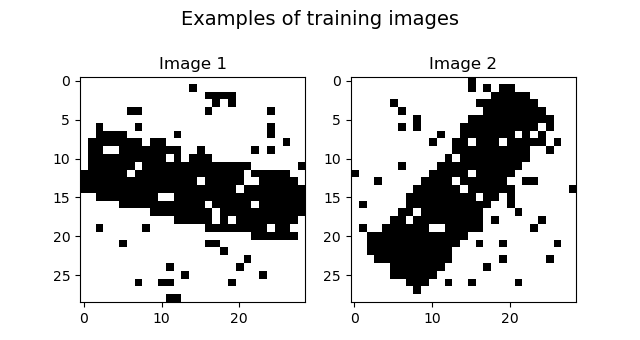
\includegraphics[width=\linewidth]{figures/angleNetwork/trainingImages.png}
  \caption{Two examples of the generated training data in this experiment.}
  \label{fig:angleImages}
\end{figure}

\paragraph{Neuron model}

As in \citet{nessler} the input neurons X are firing according to a poisson process with an average firing rate of 20 Hz when active and with 0 Hz when in an inactive state. The excitatory post synaptic potentials (EPSPs) $x_i(t)$ that these neurons produce can be seen in Figure \ref{fig:XSpike}. A double exponential kernel was used to generate the EPSP. The time constant for the rise of the signal $\tau_{rise}$ was 1 ms and the time constant for the decay of the signal $\tau_{decay}$ was 15 ms. The addition of the time step size $\delta t$ was necessary to get the time t at the end of the current simulation step. $t_f$ is the time at which the spike of $x_i$ occurred
\begin{equation}
\label{eqn:EPSP}
x_i(t) = e^{-(t + \delta t - t_f) / \tau_{decay}} - e^{-(t + \delta t - t_f) / \tau_{rise}}.
\end{equation}


\begin{figure}
  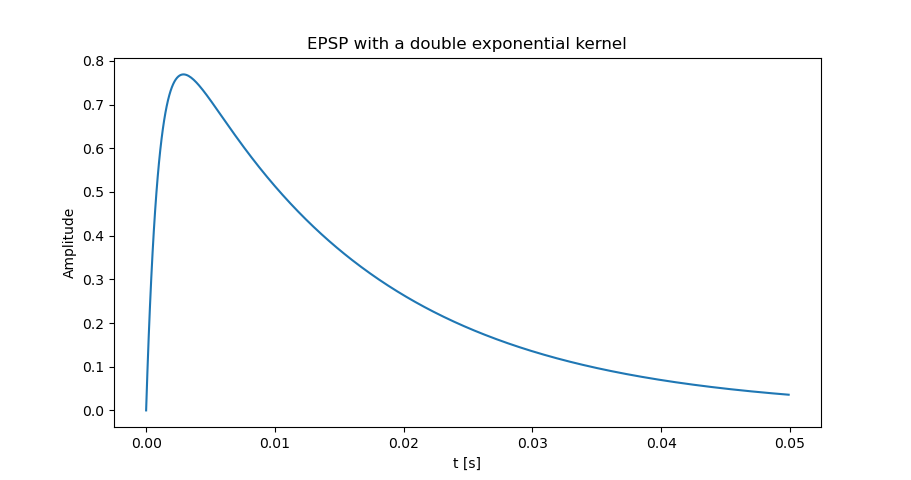
\includegraphics[width=\linewidth]{figures/XSpike.png}
  \caption{Form of an excitatory post synaptic potential generated by an input neuron over time. A double exponential kernel was used to generate this signal. These signals are fed to the next layer of the network. }
  \label{fig:XSpike}
\end{figure}

The firing rate of an output neuron $y_k$ depends exponentially on its membrane potential $u_k$ and the inhibitory signal I(t) it receives 
\begin{equation}
\label{eqn:rk}
r_k(t) = e^{u_k(t) - I(t)}.
\end{equation}
The probability of an individual output neuron to fire within a time step $\delta t$ is given by
\begin{equation}
\label{eqn:rkdt}
r_k(t) \cdot \delta t.
\end{equation}

\paragraph{Network architecture}
Each pixel of an input image was connected to two neurons. The first of these neurons is in an active state when the pixel is black and in an inactive state otherwise. The second neuron expresses the opposite behaviour. As a consequence the network needs 1682 ($29 \cdot 29 \cdot 2$) excitatory input neurons $x_1,...,x_n$. These input neurons are fully connected to ten excitatory output neurons $y_1,...,y_k$. This means that that every input neuron $x_i$ is connected to each output neuron $y_k$. The membrane potential $u_k$ of each output neuron is calculated by multiplying the EPSP of each input neuron times the weight of the connection between the input and output neuron 
\begin{equation}
\label{eqn:uk}
u_k(t) = \sum_{i=1}^n w_{ki} \cdot x_i(t).
\end{equation}
In \citet{nessler} each output neuron $y_k$ also had an intrinsic excitability $w_{k0}$ which was learned for each neuron. For this experiment however it was omitted, as each orientation of input images was equally likely, thus the intrinsic excitability of each output neuron would end up being the same.

The output neurons are modelled in a winner-takes-all (WTA) circuit. This means that whenever one output neuron spikes, a lateral inhibitory signal is fed to all output neurons, thus preventing the further activation of them for $\sigma_{inh} = 5 ms$. After completion of the training of the network each output neuron should be active for bars in a coherent area. Each of those areas should ideally be of equal size. As the bars can be oriented between 0 and 359 degrees, but each 180 degree rotation of an image results in an equivalent image, the desired size of the active area of an output neuron should be 18 degrees.


\paragraph{Inhibition}
The inhibition signal was chosen to depend on the current membrane potential of the output neurons. According to \citet{nessler} the total firing rate of the output neurons is
\begin{equation}
\label{eqn:R}
R(t) = \sum_{k=1}^K e^{u_k(t) - I(t)}.
\end{equation}
Solving this equation for I(t) yields
\begin{equation}
\label{}
R(t) = \frac{ \sum_{k=1}^K e^{u_k(t)}}{e^{I(t)}}
\end{equation}
\begin{equation}
\label{}
e^{I(t)} = \frac{\sum_{k=1}^K e^{u_k(t)}}{R(t)}
\end{equation}
\begin{equation}
\label{}
I(t) = \ln{ \frac{ \sum_{k=1}^K e^{u_k(t)}}{R(t)}}
\end{equation}
\begin{equation}
\label{eqn:I(t)}
I(t) =  - \ln{R(t)} + \ln{  \sum_{k=1}^K e^{u_k(t)}}.
\end{equation}
When implementing the inhibition the $- \ln{R(t)}$ term of Equation \ref{eqn:I(t)} was overlooked, that means it was assumed to be zero. Because of that R(t) equals 1 when the inhibition is active. This error was not detected at first, as the chance that a Y neuron fires within a time step of 1 ms with active inhibition is 1/1000 due to that oversight.

Whenever an output neuron produces a spike the inhibition signal I(t) is subtracted from the membrane potential Uk(t) of every output neuron. This happens for the duration of $\sigma_{inh} = 5 ms$. Thus follows

\begin{equation}
\label{eqn:iinh}
I(t) = \begin{dcases*} \ln ( \sum_{i=1}^k e^{u_k} ) & if any $y_k$ fired in $ [t^f, t^f  + \sigma_{inh}] $ \\
0 & \text{if any $y_k$ did not fire in $ [t^f, t^f + \sigma_{inh}] $. } \end{dcases*}\end{equation}

\paragraph{Spike timing dependent plasticity}
The weights $w_{ki}$ between neurons $x_i$ and $y_k$ are updated whenever an output neuron fires. The time window $\sigma$ was set to 10 ms according to \citet{nessler}. If $y_k$ produces a spike all its weights are updated as
\begin{equation}
\label{deltawki}
\Delta w_{ki} = \begin{dcases*} \lambda \cdot (ce^{-w_{ki}} - 1) & if $x_{i}$ fired in $ [t^f - \sigma, t^f] $ \\
\lambda \cdot (-1) & \text{if $ x_i $ did not fire in $ [t^f - \sigma, t^f] $, } \end{dcases*}
\end{equation}
where $\lambda$ is the learning rate, the parameter c shifts the weight values, $t^f$ is the time when $y_k$ spiked and $\sigma$ is the time window in which input spikes are considered as "before" an output spike. As the membrane potentials $u_k$ of the output neurons result from the addition of the EPSPs of the 1682 input neurons times the corresponding weight, a way to control the average size of u is needed. If u is to small the output neurons will fire too sparsely and if u is too big it will impair the learning process. So to limit u, the size of the weights is controlled via the parameter c. The learning rate $\lambda$ is needed to control the size of each weight update. If it is too big few output neurons will take over more than the expected 18° areas and others will only respond for smaller areas or not at all. On the other hand if $\lambda$ is too small the network will learn very slowly and may never converge. Due to these two parameters being unwieldy to determine analytically they were chosen via grid search. 


\subsection{Results}

\paragraph{Parameter search}
The two parameters c, which controls the size of the weights, and the learning rate $\lambda$ were fitted to the network via grid search.	The tested parameters were as follows:
\begin{itemize}
  \item $c = 1$ ($\lambda = 10^{-2}, 10^{-3}, 10^{-4}$) 
  \item $c = 10$ ($\lambda = 10^{-2}, 10^{-3}, 10^{-4}$) 
  \item $c = 20$ ($\lambda = 10^{-2}, 10^{-2.5}, 10^{-3}, 10^{-3.5},  10^{-4}, 10^{-4.5}, 10^{-5}$) 
  \item $c = 30$ ($\lambda = 10^{-2}, 10^{-2.5}, 10^{-3}, 10^{-3.5}$) 
\end{itemize}
The simulation was conducted by simulating small discrete time steps and calculating the changes of the network in each step. The step size $\delta t$ was chosen as 1 ms.

\paragraph{$c = 1$}
The best results for $c = 1$ were achieved with $\lambda = 10^{-2}$. But overall this value for c did not work, even tough the network did learn to cluster images into eight groups depending on their orientation. In Figure \ref{fig:c1Pie} one can see which output neuron was the most active during the training process for each angle in 1° steps.

\begin{figure}
  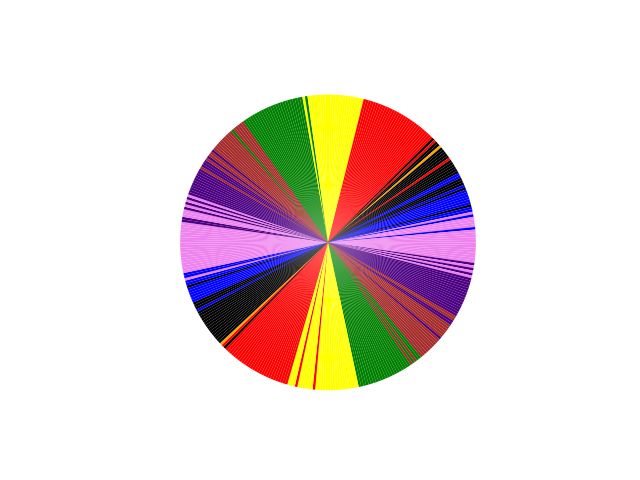
\includegraphics[width=\linewidth]{figures/angleNetwork/c1Pie.png}
  \caption{Most active output neuron depending on orientation of the training image during the training process. $c = 1, \lambda = 10^{-2}$}
  \label{fig:c1Pie}
\end{figure}

In Figure \ref{fig:c1Distinct} the training progress of the network can be seen. The figure shows the number of distinct output neurons active during the presentation of each training image shown. Due to the large, compared to other values of c, learning rate the network learned quickly. However after iteration 70 there were images shown for which not a single output neuron spiked. This dying out of the networks activity is due to the parameter c being too small, which leads to too low membrane potentials.

\begin{figure}
  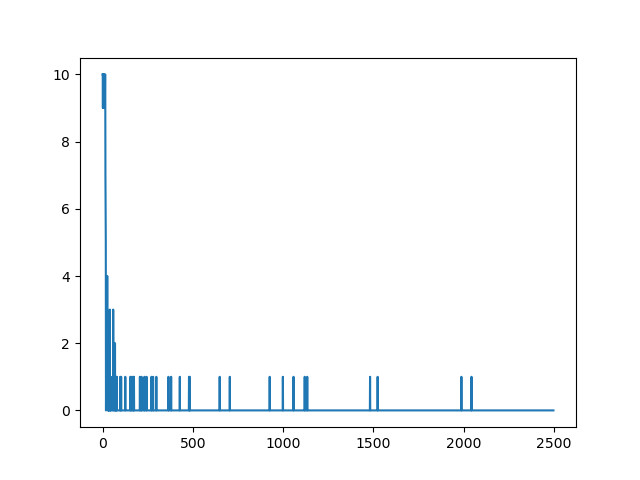
\includegraphics[width=\linewidth]{figures/angleNetwork/c1Distinct.png}
  \caption{Number of distinct output neurons active during the presentation duration of each training image. x-axis: image shown, y-axis: distinct output neurons active, $c = 1, \lambda = 10^{-2}$}
  \label{fig:c1Distinct}
\end{figure}

\paragraph{$c = 10$}
This value of $c = 10$ had the same problem of the network activity dying out as $c = 1$ although at a later point in time, as can be seen in Figure \ref{fig:c10Distinct}. Also in Figure \ref{fig:c10LastSpikes} the last 50 output spikes of the training process can be seen. As indicated by Figure \ref{fig:c10Distinct} the activity is sparse.

\begin{figure}
  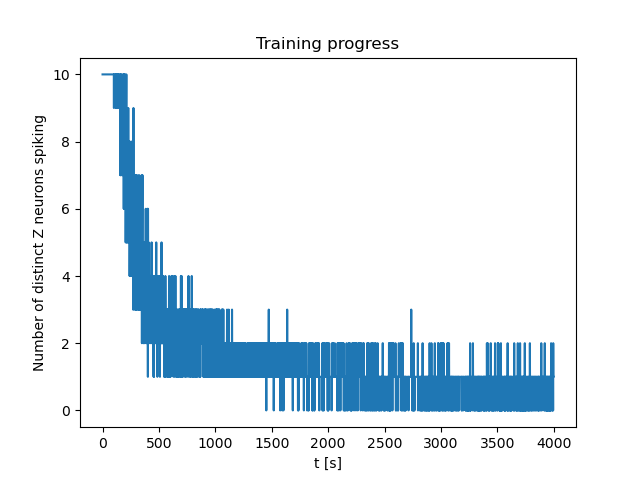
\includegraphics[width=\linewidth]{figures/angleNetwork/c10_3distinctZ.png}
  \caption{Number of distinct output neurons active during the presentation duration of each training image. x-axis: image shown, y-axis: distinct output neurons active, $c = 10, \lambda = 10^{-3}$}
  \label{fig:c10Distinct}
\end{figure}

\begin{figure}
  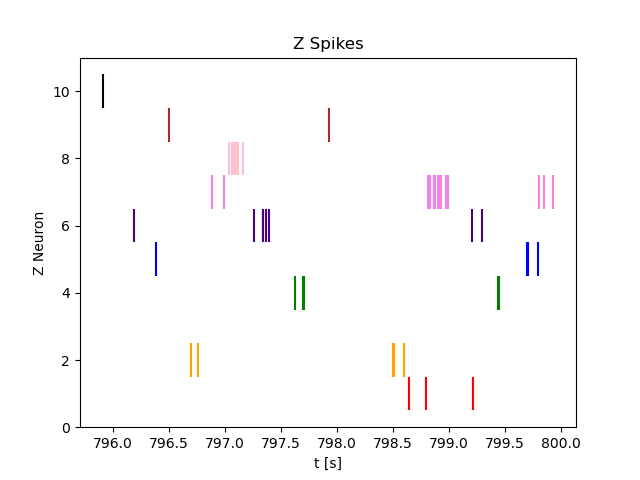
\includegraphics[width=\linewidth]{figures/angleNetwork/c10_3_50LastZSpikes.png}
  \caption{Last 50 output neuron spikes, $c = 10, \lambda = 10^{-3}$}
  \label{fig:c10LastSpikes}
\end{figure}

\paragraph{$c = 20$}
$c = 20$ was the first value for which the network activity did not die out after some time. For $\lambda = 10^{-2}$ one output neuron learned to spike first for every possible input image orientation, see Figure \ref{fig:c20_2Pie}. 

\begin{figure}
  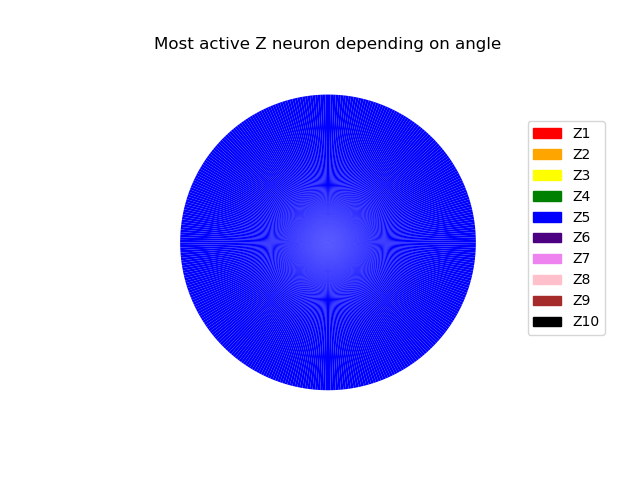
\includegraphics[width=\linewidth]{figures/angleNetwork/c20_2pie.png}
  \caption{Most active output neuron depending on orientation of the training image during the training process. $c = 20, \lambda = 10^{-2}$}
  \label{fig:c20_2Pie}
\end{figure}

With $c = 20$ and $\lambda = 10^{-3}$ the first combination that yielded a stable network was found. In Figure \ref{fig:c20_3Distinct} the amount of distinct output neurons firing during the presentation of each training image can be seen. Figure \ref{fig:c20_3averageZ} shows the proportion of the most active output neuron to all other output neurons active for each training image. Both of these figures can be used to measure the training progress of the network. Figure \ref{fig:c20_3averageZ} however shows the additional information how certain the network is that a training image belongs to a specific group.

\begin{figure}
  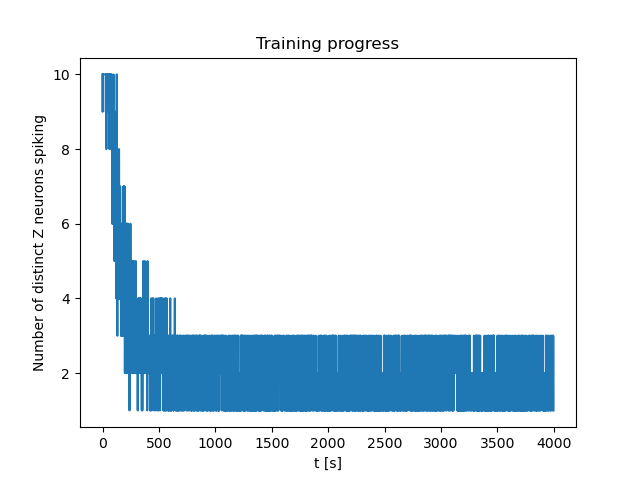
\includegraphics[width=\linewidth]{figures/angleNetwork/c20_3distinctZ.png}
  \caption{Number of distinct output neurons active during the presentation duration of each training image. x-axis: image shown, y-axis: distinct output neuron active, $c = 20, \lambda = 10^{-3}$}
  \label{fig:c20_3Distinct}
\end{figure}

\begin{figure}
  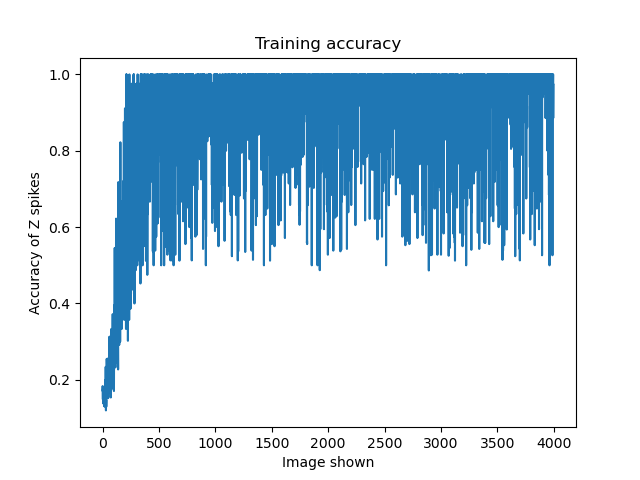
\includegraphics[width=\linewidth]{figures/angleNetwork/c20_3averageZ.png}
  \caption{Proportion (accuracy) of most active output neuron  to activity of all other output neurons during the presentation duration of each training image. $c = 20, \lambda = 10^{-3}$}
  \label{fig:c20_3averageZ}
\end{figure}

As this network did not die out after some time the trained network was analysed further. 180 images were generated in 1° steps and each was shown to the network for 200 ms. During each image presentation duration the most active output neuron was recorded. This yielded Figure \ref{fig:c20_3Pie}.

\begin{figure}
  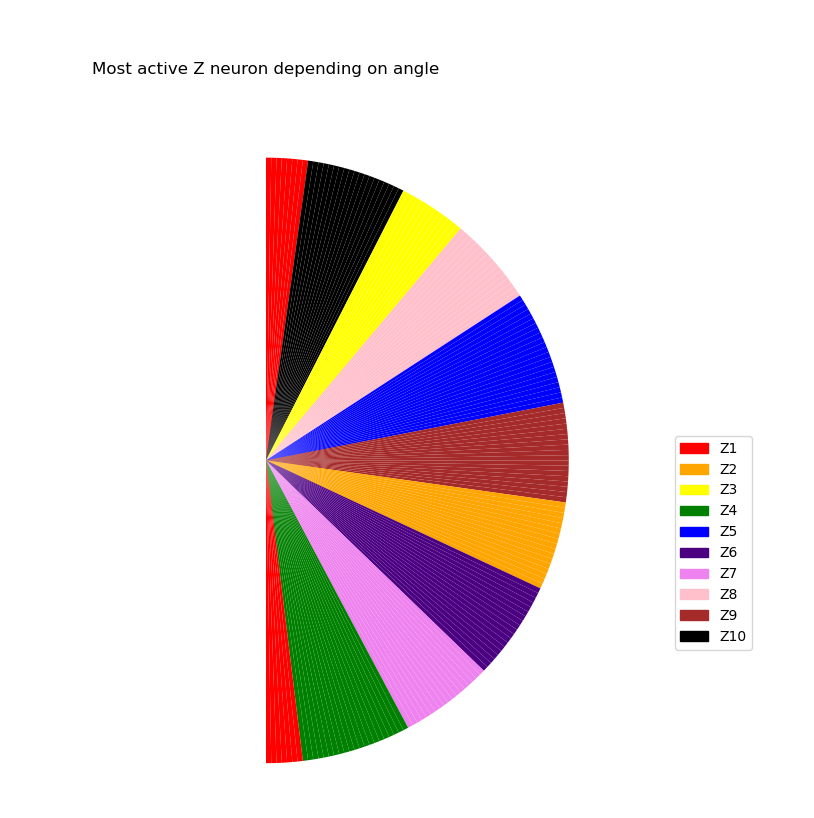
\includegraphics[width=\linewidth]{figures/angleNetwork/c20_3validationPie.png}
  \caption{Most active output neuron depending on orientation of the training image during the training process. $c = 20, \lambda = 10^{-3}$}
  \label{fig:c20_3Pie}
\end{figure}

Also the number of distinct output neurons firing during each image presentation was recorded and is shown in \ref{fig:c20_3validationDistinctZSpikes}. In this figure it seems that the points in which there are three distinct output neurons active are periodic in nature. This can be explained by Figure \ref{fig:c20_3validationZSpikes}. There it can be seen that whenever the image orientation nears the border between two competing output neurons both start to be active. This explains why for large parts of Figure \ref{fig:c20_3validationDistinctZSpikes} 2 neurons are active, as large portions of the bar in the image is overlapping the areas of the two nearest output neurons, thus producing high membrane potentials for both. The third distinct output neuron that is occasionally active seems to be of stochastic nature as much of the bars in the images overlaps areas of all other output neurons, thus generating a non zero membrane potential for each output neuron. However the occurrence of 3 distinct active output neurons seems to mostly occur at or close to the border between two competing output neurons, as there are already 2 distinct neurons firing by design.

\begin{figure}
  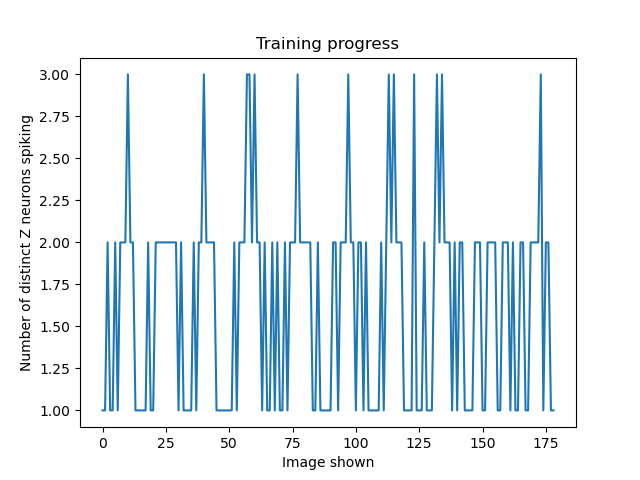
\includegraphics[width=\linewidth]{figures/angleNetwork/c20_3validationDistinctZSpikes.png}
  \caption{Number of distinct output neurons active during the presentation duration of each training image. x-axis: image shown, y-axis: distinct output neuron active, $c = 20, \lambda = 10^{-3}$}
  \label{fig:c20_3validationDistinctZSpikes}
\end{figure}

\begin{figure}
  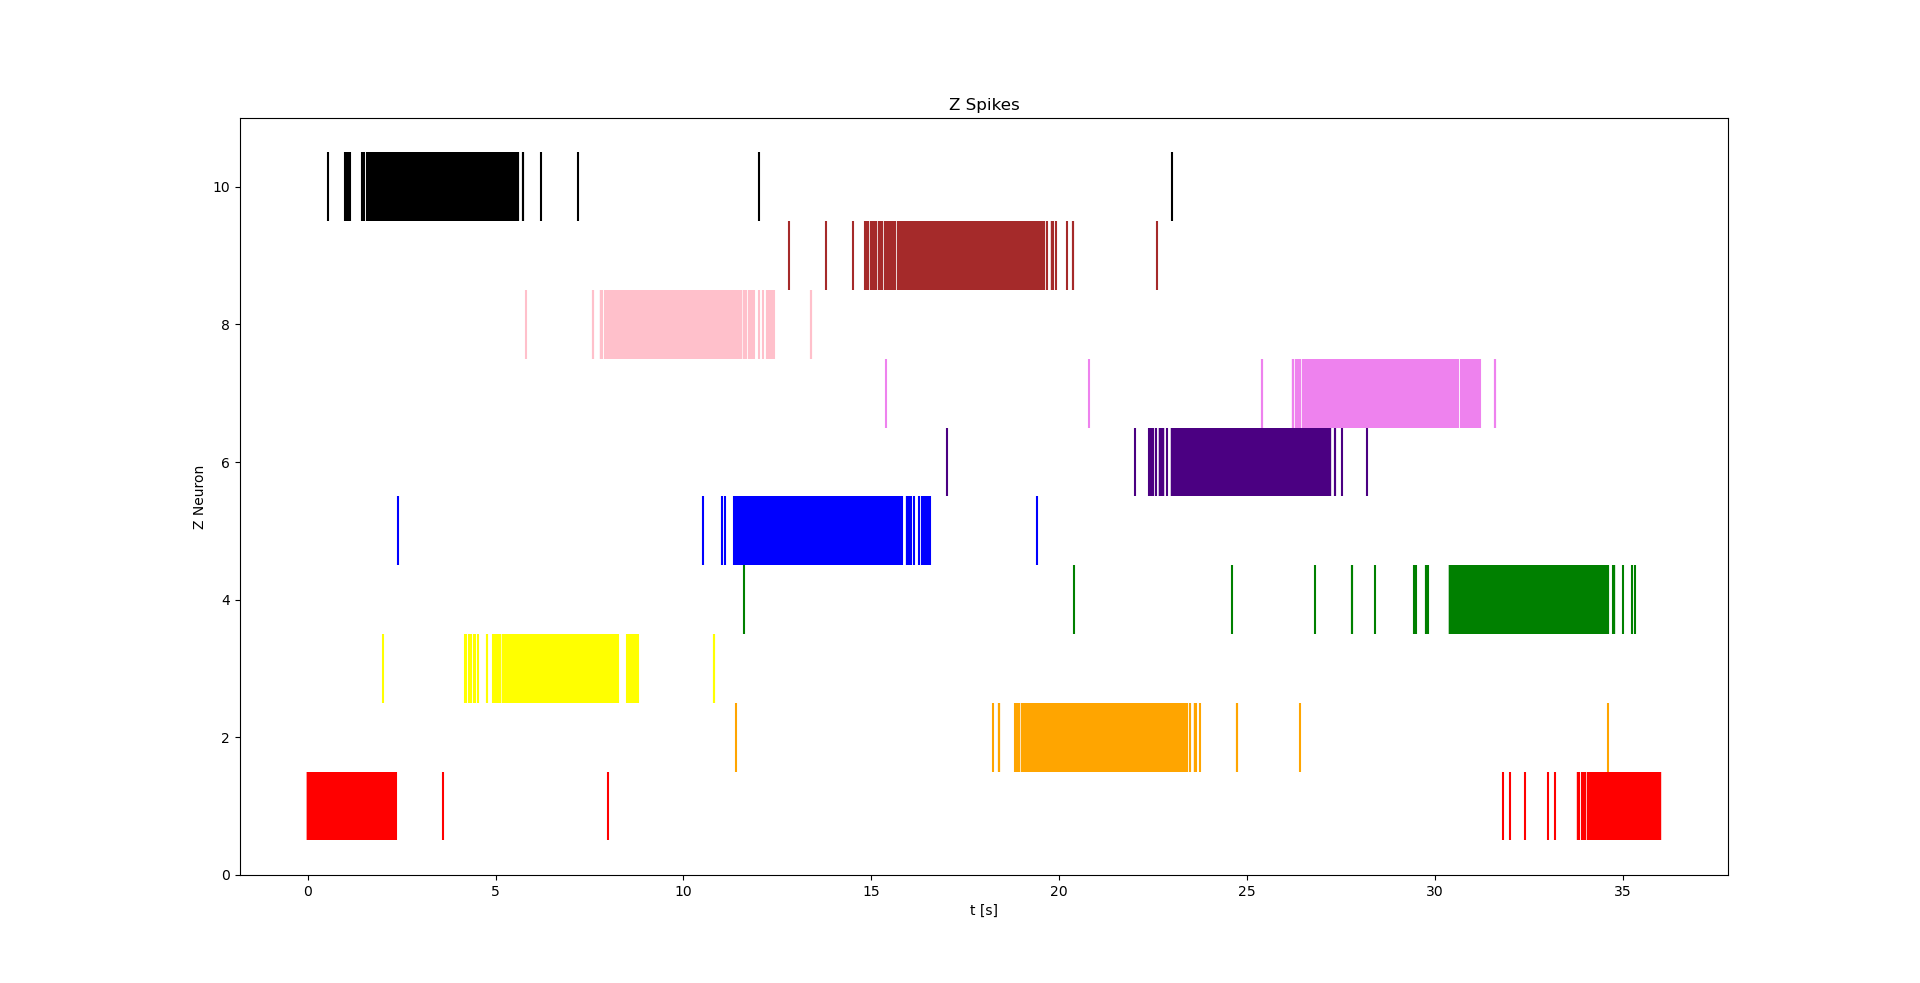
\includegraphics[width=\linewidth]{figures/angleNetwork/c20_3validationZSpikes.png}
  \caption{Output spikes over the presentation of input images from 0 to 179°, $c = 20, \lambda = 10^{-3}$}
  \label{fig:c20_3validationZSpikes}
\end{figure}

Also it was possible to project the learned weights $w_{ki}$ into the 2-D space to observe what they represent. This projection can be seen in Figure \ref{fig:c20_3weights2.png} for the weights of $y_{10}$.

\begin{figure}
  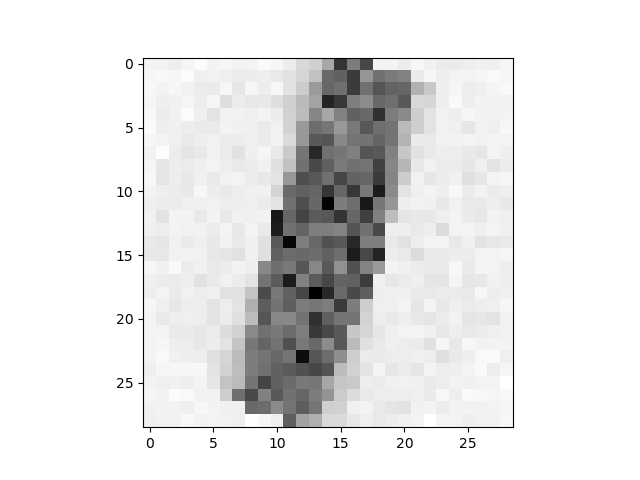
\includegraphics[width=\linewidth]{figures/angleNetwork/c20_3weights2.png}
  \caption{Visualization of the learned weights of $y_{10}$.}
  \label{fig:c20_3weights2.png}
\end{figure}

The results for smaller $\lambda$ were also valid, but they did not seem to yield superior results to the parameters $c = 20$ and $\lambda = 10^{-3}$. As with smaller learning rates the training simply took longer and the performance of the network did not improve they were discarded and  the learning rate $\lambda = 10^{-3}$ was declared winner for $c = 20$. To save space the figures of smaller learning rates will not be shown here.

\paragraph{$c = 30$}
also yielded a functioning network, but it did perform analogous to $c = 20$. It did perform in the same way, as with $c = 20$ the output neurons already fire every 5 ms, slowed down by the inhibition. By increasing c further the output neurons did not increase their activity.

\subsection{Conclusion}

The parameters $c = 20$ and $\lambda = 10^{-3} $ were finally chosen as the network performed the best and trained the quickest with these parameters, without raising the membrane potential needlessly.

\section{Experiment 2: Horizontal and vertical bars}
\label{section:horvert}

 \subsection{Introduction}

For this experiment the impact of a neuron layer that encodes a-priori information should be analysed.

\subsection{Methods}

\paragraph{Input data}
29 x 29 black and white images with either horizontal or vertical oriented bars on them were used, as it was more straightforward to express a-priori information. The orientation of the training images was chosen randomly via a uniform distribution. Also the positions of the bars in the images were uniformly distributed. The rest of the image generation process is analogous to experiment 1, except no circular mask was used. Examples of the input data can be seen in Figure \ref{fig:horvertImages}. To show the value of the a-priori information validation images with two bars forming a cross were also generated, seen in Figure \ref{fig:horvertTrainingCrossImage}. When shown to the network in the validation process the prior neurons were given the information that a cross is either in horizontal or vertical orientation.

\begin{figure}
  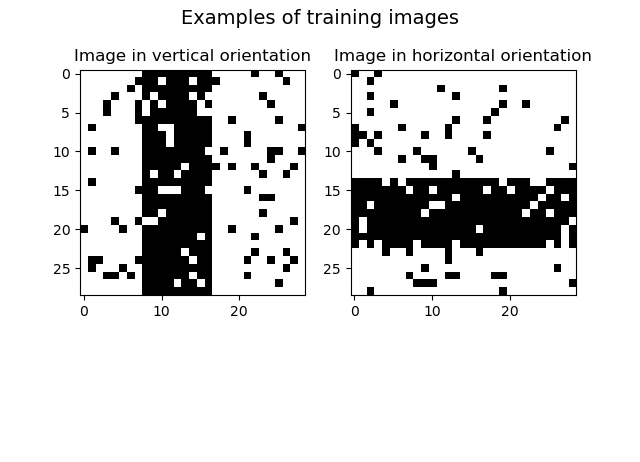
\includegraphics[width=\linewidth]{figures/horvert/horvertTrainingImages.png}
  \caption{Training images generated for experiment 2. One image of each possible orientation at a random position.}
  \label{fig:horvertImages}
\end{figure}

\begin{figure}
  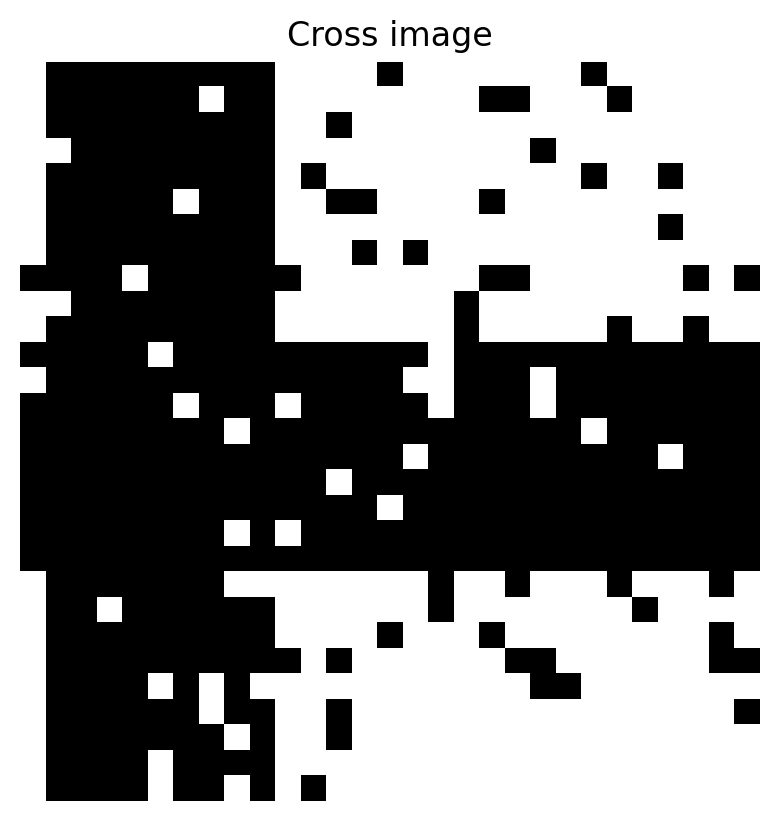
\includegraphics[width=0.6\linewidth]{figures/horvert/horvertTrainingCrossImage.png}
  \caption{Generated cross image which can represent either horizontal or vertical orientation.}
  \label{fig:horvertTrainingCrossImage}
\end{figure}


\paragraph{Network architecture}

This experiment used a expanded version of the network used in experiment 1. An additional layer of prior neurons $z_1,z_2$ was added. Whenever an image was oriented vertically $z_1$ was active and $z_2$ was inactive. For horizontal orientations $z_2$ was active and $z_1$ was inactive. Prior neurons in an active state had a firing frequency of 50 Hz and fired with 0 Hz when inactive.

\paragraph{Neuron model}
The input and output neurons functioned the same way as in the previous experiment. The prior neurons fire according to a poisson process with their firing rate. Each prior neuron $Z_l$ is connected to every output neuron $Y_k$ and thus has weights $w_{kl}$ that were learned by the network. 

\paragraph{Parameters}
As the amount of input neurons and the average number of black pixels in an input image stayed roughly the same in this experiment, the same parameters $c=  20$ and $\lambda = 10^{-3}$ could be used. However as there are only two prior neurons, a way to amplify their produced signals was needed, otherwise their impact on the membrane potential of the output neurons would not be distinctive enough. So the EPSPs $z_l(t)$ were multiplied by the factor $Z_{factor}$. This factor was determined via grid search. The additional prior layer resulted in an expanded version of the membrane potential $u_k(t)$

\begin{equation}
\label{eqn:ukHorvert}
u_k(t) = \sum_{i=1}^n w_{ki} \cdot x_i(t) + w_{kl} \cdot Z_{factor} \cdot z_l(t).
\end{equation}

\subsection{Results} 

The following values for $Z_{factor} $ were tried with $c = 20$ and $\lambda = 10^{-3}$:
\begin{itemize}
  \item $Z_{factor} = 3$
  \item $Z_{factor} = 5$
  \item $Z_{factor} = 7$  
  \item $Z_{factor} = 10$ 
  \item $Z_{factor} = 20$
\end{itemize}

For $Z_{factor} = 10$ and $20$ the prior neurons impacted the learning progress negatively and let single prior neurons respond to too much area. An example of this can be seen in Figure \ref{fig:horvert_c20_3_Zfactor20_horizontalLines}

\begin{figure}
  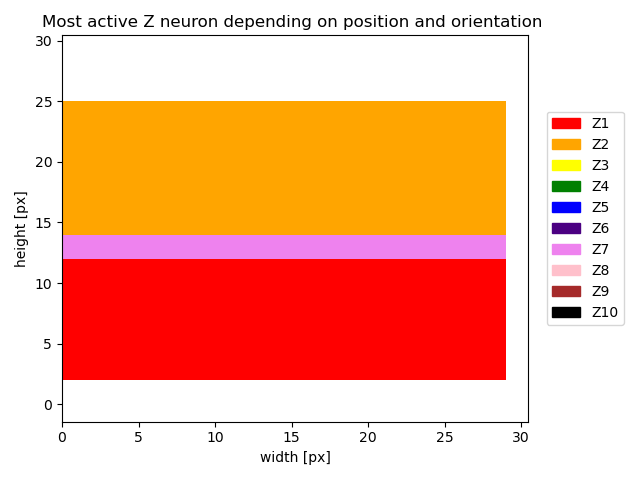
\includegraphics[width=\linewidth]{figures/horvert/horvert_c20_3_Zfactor20_horizontalLines.png}
  \caption{Most active output neuron for horizontal orientation and position on the y-axis of the training image during the training process. $c = 20, \lambda = 10^{-3}, Z_{factor} = 20$}
  \label{fig:horvert_c20_3_Zfactor20_horizontalLines}
\end{figure}


The best results were achieved with $Z_{factor} = 5$. When looking at the training progress in Figure \ref{fig:horvert_c20_3_Zfactor5_averageZ} it can be seen that the training accuracy is higher compared to experiment 1. This is due to the added a-priori information and the fact that less of each bar in an image is overlapping with multiple areas of output neurons. The network activity at the end of the training process can be seen in Figure \ref{fig:horvertLastSpikes}. In Figures \ref{fig:horvert_c20_3_Zfactor5_horizontalLines} and \ref{fig:horvert_c20_3_Zfactor5_verticalLines} the most active output neuron of the trained network is plotted for horizontal bars in every position and in the second plot for vertical bars in every position. Every one of the ten output neurons responds primarily to one coherent area in one orientation. The values of the learned prior weights $w_{kl}$ were plotted in Figures \ref{fig:wkl1} and \ref{fig:wkl2}. In these figures, in combination with Figures \ref{fig:horvert_c20_3_Zfactor5_horizontalLines} and \ref{fig:horvert_c20_3_Zfactor5_verticalLines}, can be seen that each prior neuron specialized on one orientation.

\begin{figure}
  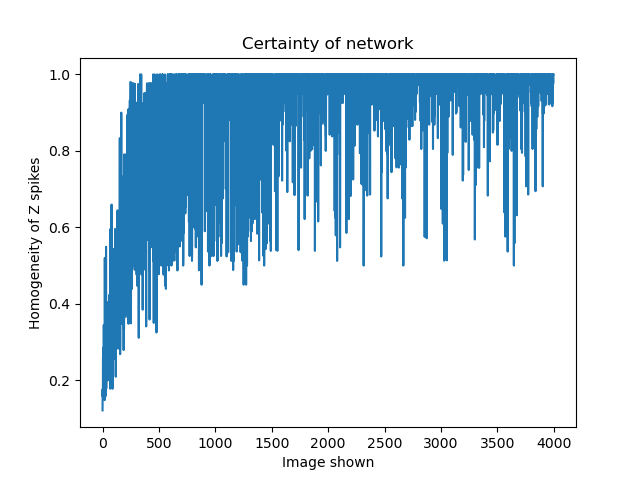
\includegraphics[width=\linewidth]{figures/horvert/horvert_c20_3_Zfactor5_averageZ.png}
  \caption{Proportion (accuracy) of most active output neuron  to activity of all other output neurons during the presentation duration of each training image. $c = 20, \lambda = 10^{-3}, Z_{factor} = 5$}
  \label{fig:horvert_c20_3_Zfactor5_averageZ}
\end{figure}

\begin{figure}
  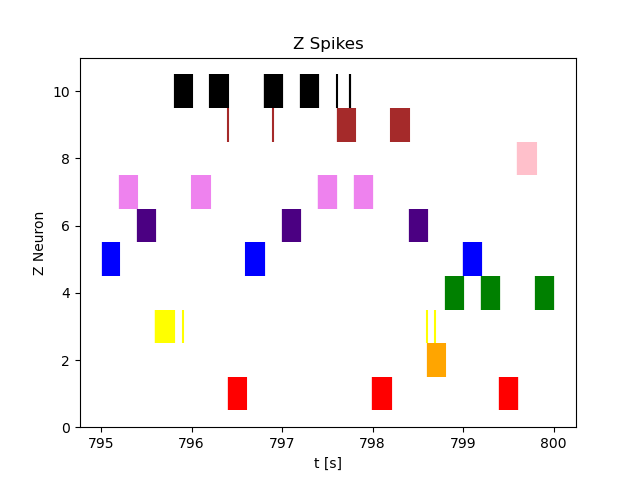
\includegraphics[width=\linewidth]{figures/horvert/horvert_c20_3_Zfactor5_1000LastZSpikes.png}
  \caption{Last 1000 output neuron spikes, $c = 20, \lambda = 10^{-3}$, $Z_{factor} = 5$}
  \label{fig:horvertLastSpikes}
\end{figure}

\begin{figure}
  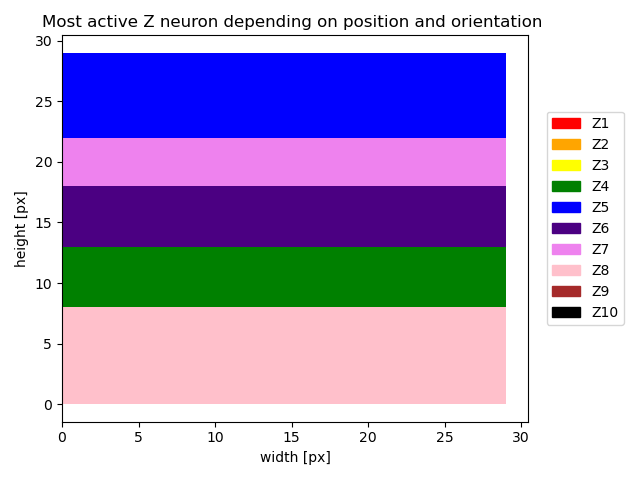
\includegraphics[width=\linewidth]{figures/horvert/horvert_c20_3_Zfactor5_horizontalLines.png}
  \caption{Most active output neuron for images of horizontal orientation and position on the x-axis of during the validation process. $c = 20, \lambda = 10^{-3}, Z_{factor} = 5$}
  \label{fig:horvert_c20_3_Zfactor5_horizontalLines}
\end{figure}

\begin{figure}
  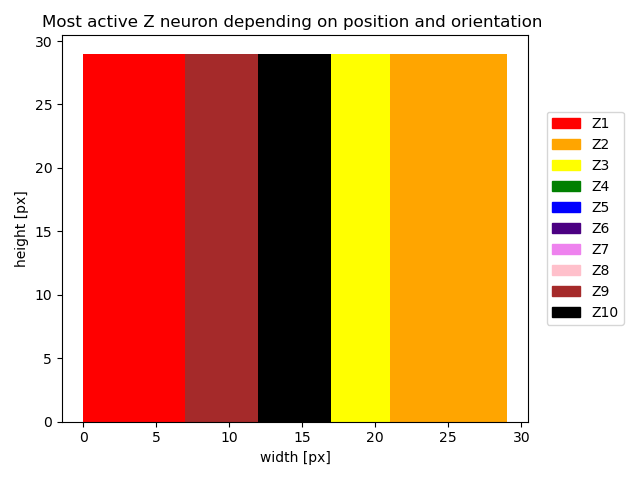
\includegraphics[width=\linewidth]{figures/horvert/horvert_c20_3_Zfactor5_verticalLines.png}
  \caption{Most active output neuron for images of vertical orientation and position on the x-axis of during the validation process. $c = 20, \lambda = 10^{-3}, Z_{factor} = 5$}
  \label{fig:horvert_c20_3_Zfactor5_verticalLines}
\end{figure}

\begin{figure}
  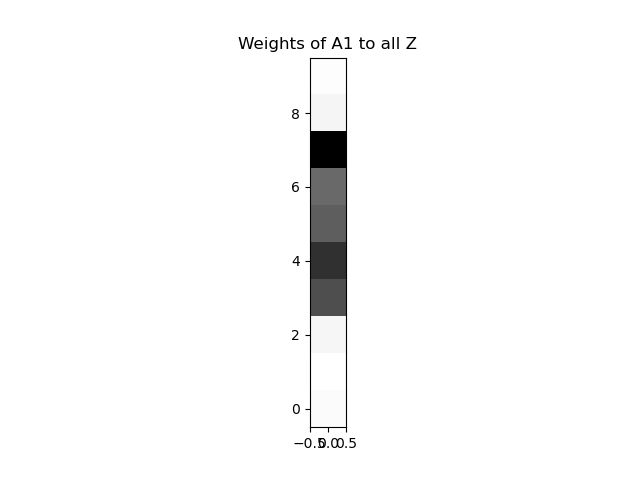
\includegraphics[width=\linewidth]{figures/horvert/horvert_c20_3_Zfactor5_priorWeight1.png}
  \caption{Values of $w_k1$, darker color means higher value. $c = 20, \lambda = 10^{-3}, Z_{factor} = 5$}
  \label{fig:wkl1}
\end{figure}

\begin{figure}
  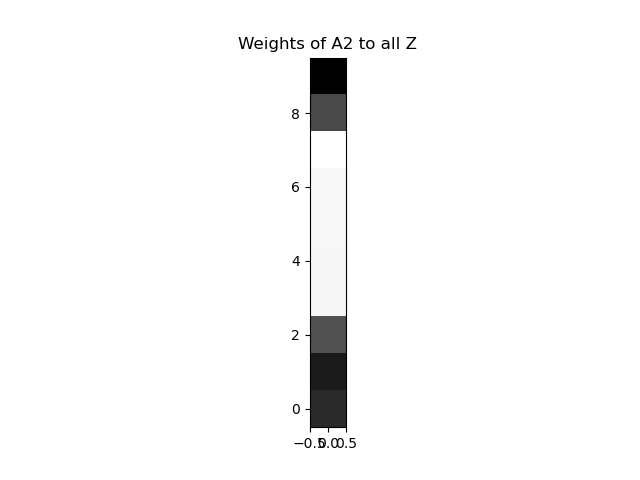
\includegraphics[width=\linewidth]{figures/horvert/horvert_c20_3_Zfactor5_priorWeight2.png}
  \caption{Values of $w_k2$, darker color means higher value. $c = 20, \lambda = 10^{-3}, Z_{factor} = 5$}
  \label{fig:wkl2}
\end{figure}

During the validation of all possible horizontal bar images the output spike activity was recorded and how many distinct output neurons were spiking during each image presentation period. For the parts where the 7 pixels high bar in the image did not overlap the areas of two output neurons only one output neuron was active. Only in the border areas there were two output neurons active. This can be seen in Figures \ref{fig:horvert_c20_3_Zfactor5_horizontalDistinctZ} and \ref{fig:horvert_c20_3_Zfactor5_horizontalZSpikes}. Compared to experiment 1 the activity is more homogeneous as each bar can only be in at most the area of four output neurons, when two of these areas are reinforced by the prior neurons.

\begin{figure}
  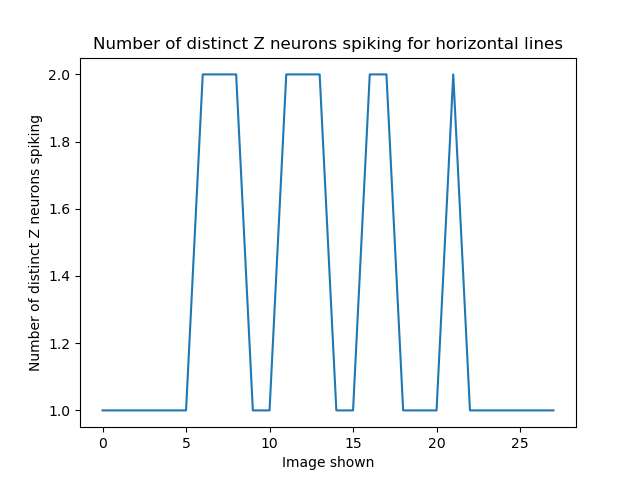
\includegraphics[width=\linewidth]{figures/horvert/horvert_c20_3_Zfactor5_horizontalDistinctZ.png}
  \caption{Distinct output neurons spiking during the presentation of all possible horizontal oriented validation images, $c = 20, \lambda = 10^{-3}$, $Z_{factor} = 5$}
  \label{fig:horvert_c20_3_Zfactor5_horizontalDistinctZ}
\end{figure}
\begin{figure}
  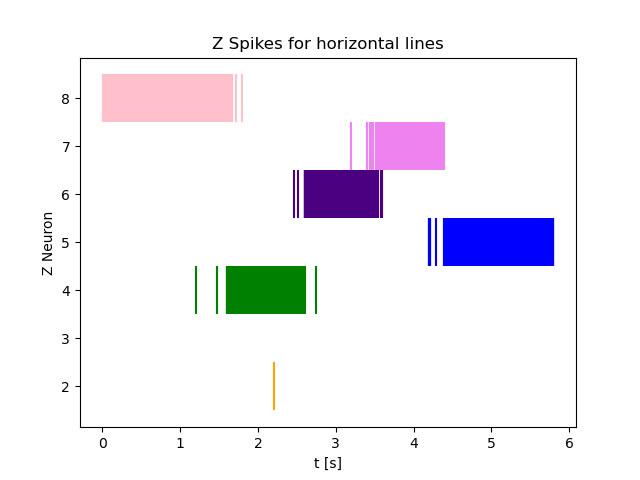
\includegraphics[width=\linewidth]{figures/horvert/horvert_c20_3_Zfactor5_horizontalZSpikes.png}
  \caption{Output neuron spikes during the presentation of all possible horizontal oriented validation images, $c = 20, \lambda = 10^{-3}$, $Z_{factor} = 5$}
  \label{fig:horvert_c20_3_Zfactor5_horizontalZSpikes}
\end{figure}


To show the impact of the prior neurons an image with two bars on it forming a cross (Figure \ref{fig:horvertValidationCross}) was generated and $z_2$ was set active indicating that the orientation is supposed to be horizontal. This resulted in the spiking pattern seen in Figure \ref{fig:horvert_c20_3_Zfactor5_crossZSpikes}. In it $Y_1$ is more active than $Y_9$ due to the influence of the prior neuron $Z_2$.

\begin{figure}
  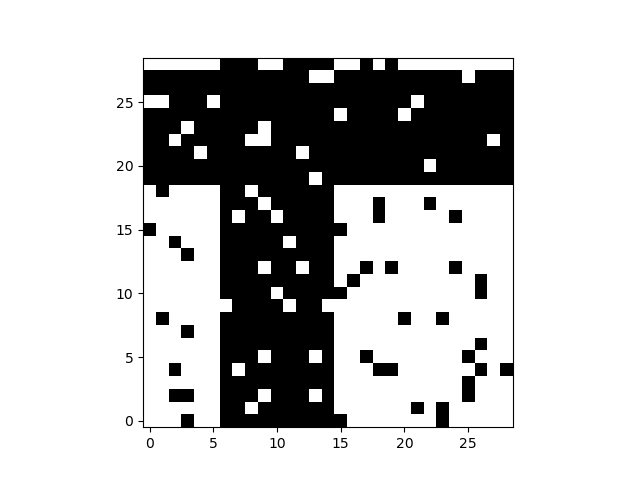
\includegraphics[width=\linewidth]{figures/horvert/horvert_c20_3_Zfactor5_validationCross.png}
  \caption{Generated validation cross image, with orientation defined as horizontal. $c = 20, \lambda = 10^{-3}, Z_{factor} = 5$}
  \label{fig:horvertValidationCross}
\end{figure}

\begin{figure}
  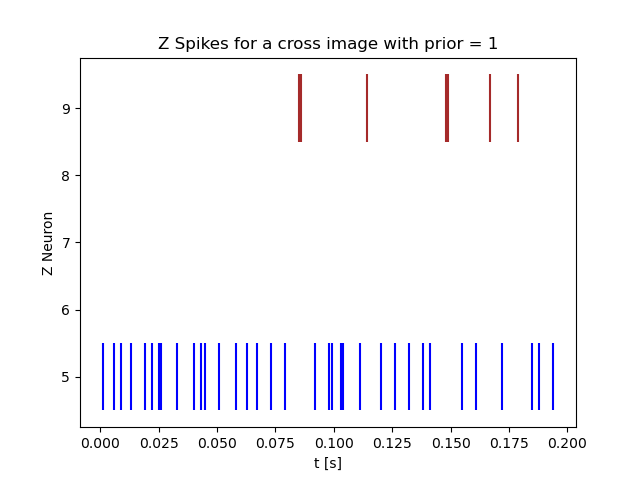
\includegraphics[width=\linewidth]{figures/horvert/horvert_c20_3_Zfactor5_crossZSpikes.png}
  \caption{Output spikes during the presentation of the validation cross image. $c = 20, \lambda = 10^{-3}, Z_{factor} = 5$}
  \label{fig:horvert_c20_3_Zfactor5_crossZSpikes}
\end{figure}



\section{Experiment 3: Rotated bars with adaptive inhibition}
\label{section:rotatedLinesAdaptiveInhibition}

\subsection{Introduction}

This experiment analyses a different approach to the implementation of the inhibition of the output neurons. 
In Experiment \ref{section:rotatedLines} and \ref{section:horvert} the output neurons were stopped from firing for a defined time window after any output neuron fired. The time window during which the inhibition was active was 5 ms, which resulted in an average output firing rate of 200 Hz. In this experiment an adaptive inhibition will be used which will regulate the membrane potentials of the output neurons so that all of them together fire with 200 Hz on average. The distinction to the previous experiments is that there never is a time window in which no output neuron may fire. Also it is assumed that the weight shifting parameter c will not be needed to be fitted to the network, as the adaptive inhibition regulates the output firing rate of the network.

\subsection{Methods}

The adaptive inhibition is given by Equation \ref{eqn:I(t)} which was already used in Experiments \ref{section:rotatedLines} and \ref{section:horvert}. However the total output firing rate $R(t)$ was set to 200 Hz in this experiment.

\subsection{Results}

Several different values for the parameter c were tested. As expected the firing rate of the output neurons 200 Hz on average regardless of the value of c. However for values of c bigger than 100 the network did not learn correctly. For those values some output neurons learned to respond to areas of more than 18°, while other neurons did not respond to any areas. For $c = 20$ the network performed equally to Experiment \ref{section:rotatedLines}. The results for that parameter can be seen in Figures \ref{fig:angleNetworkAdaptiveInhibitionTraining}, \ref{fig:angleNetworkAdaptiveInhibitionOutputFiringRate} and \ref{fig:angleNetworkAdaptiveInhibitionValidation}.


\begin{figure}
  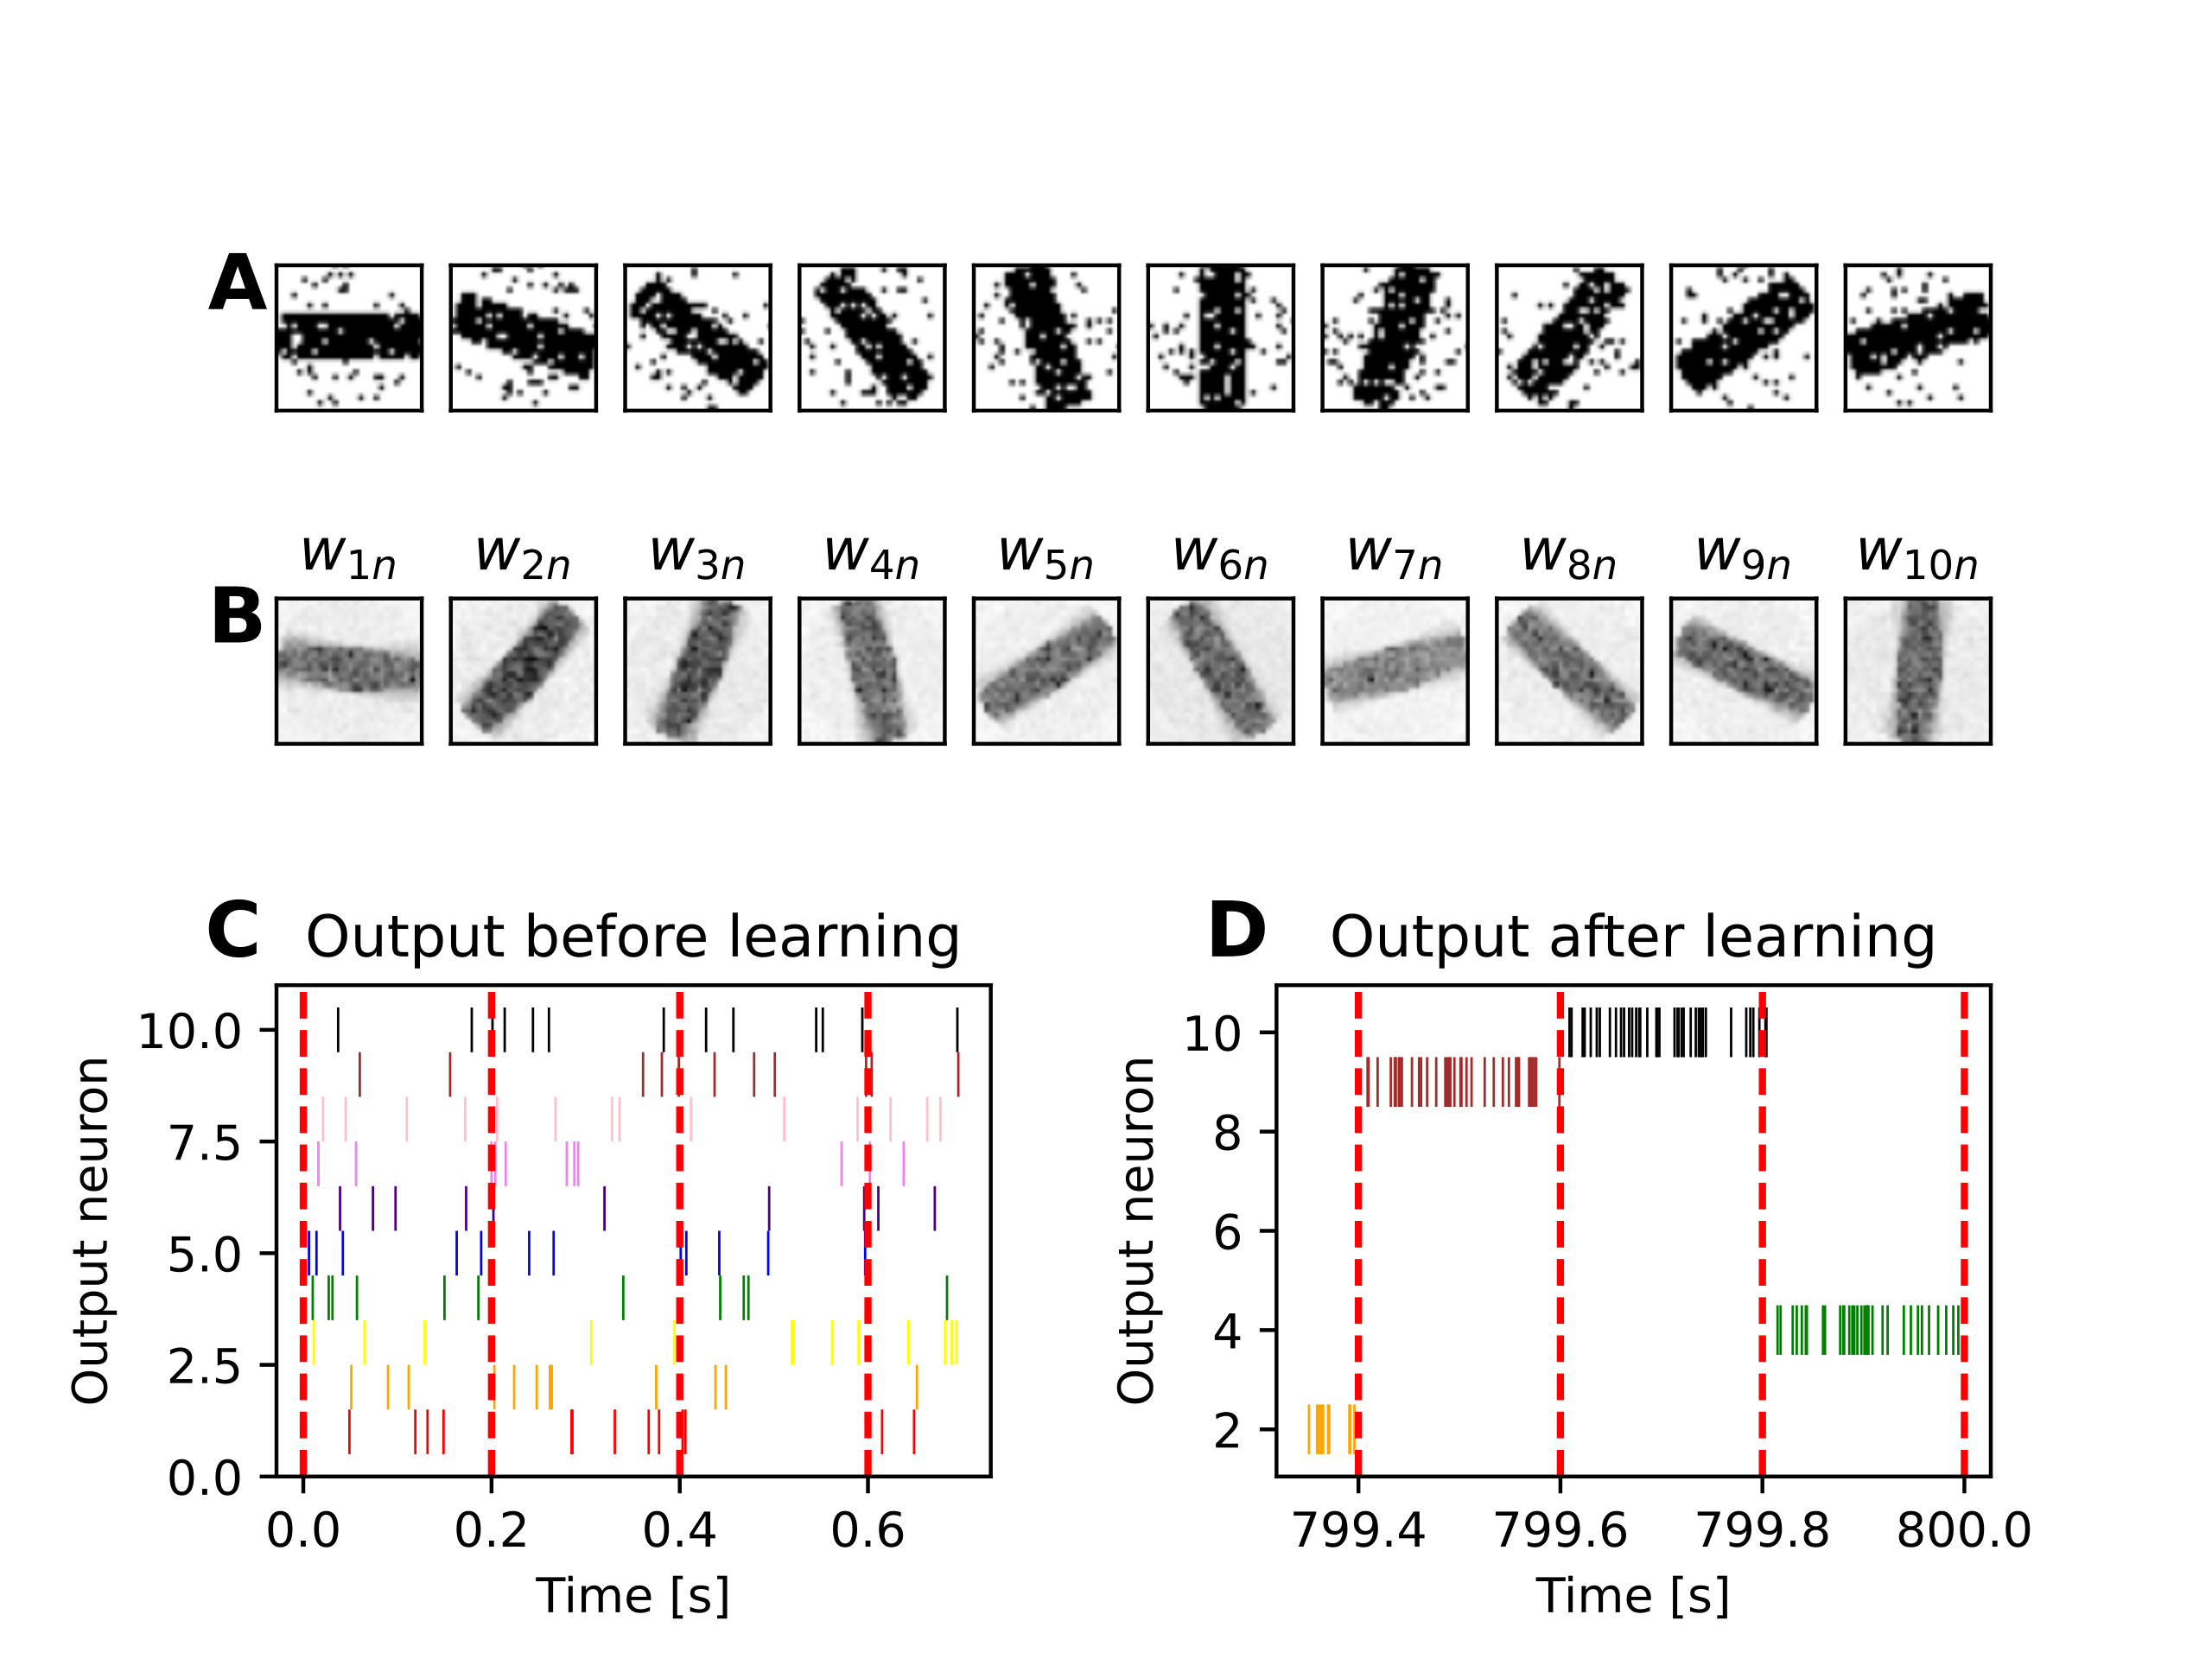
\includegraphics[width=\linewidth]{figures/angleAdaptiveInh/trainingPlot.png}
  \caption{\textbf{Training.} \textbf{A} Examples of 29 x 29-pixel input images of rotated bars and background noise. \textbf{B} Learned weights of the connections between input and output neurons. \textbf{C, D} Spike activity expressed by the output neurons before and after the training of the network. }
  \label{fig:angleNetworkAdaptiveInhibitionTraining}
\end{figure}

\begin{figure}
  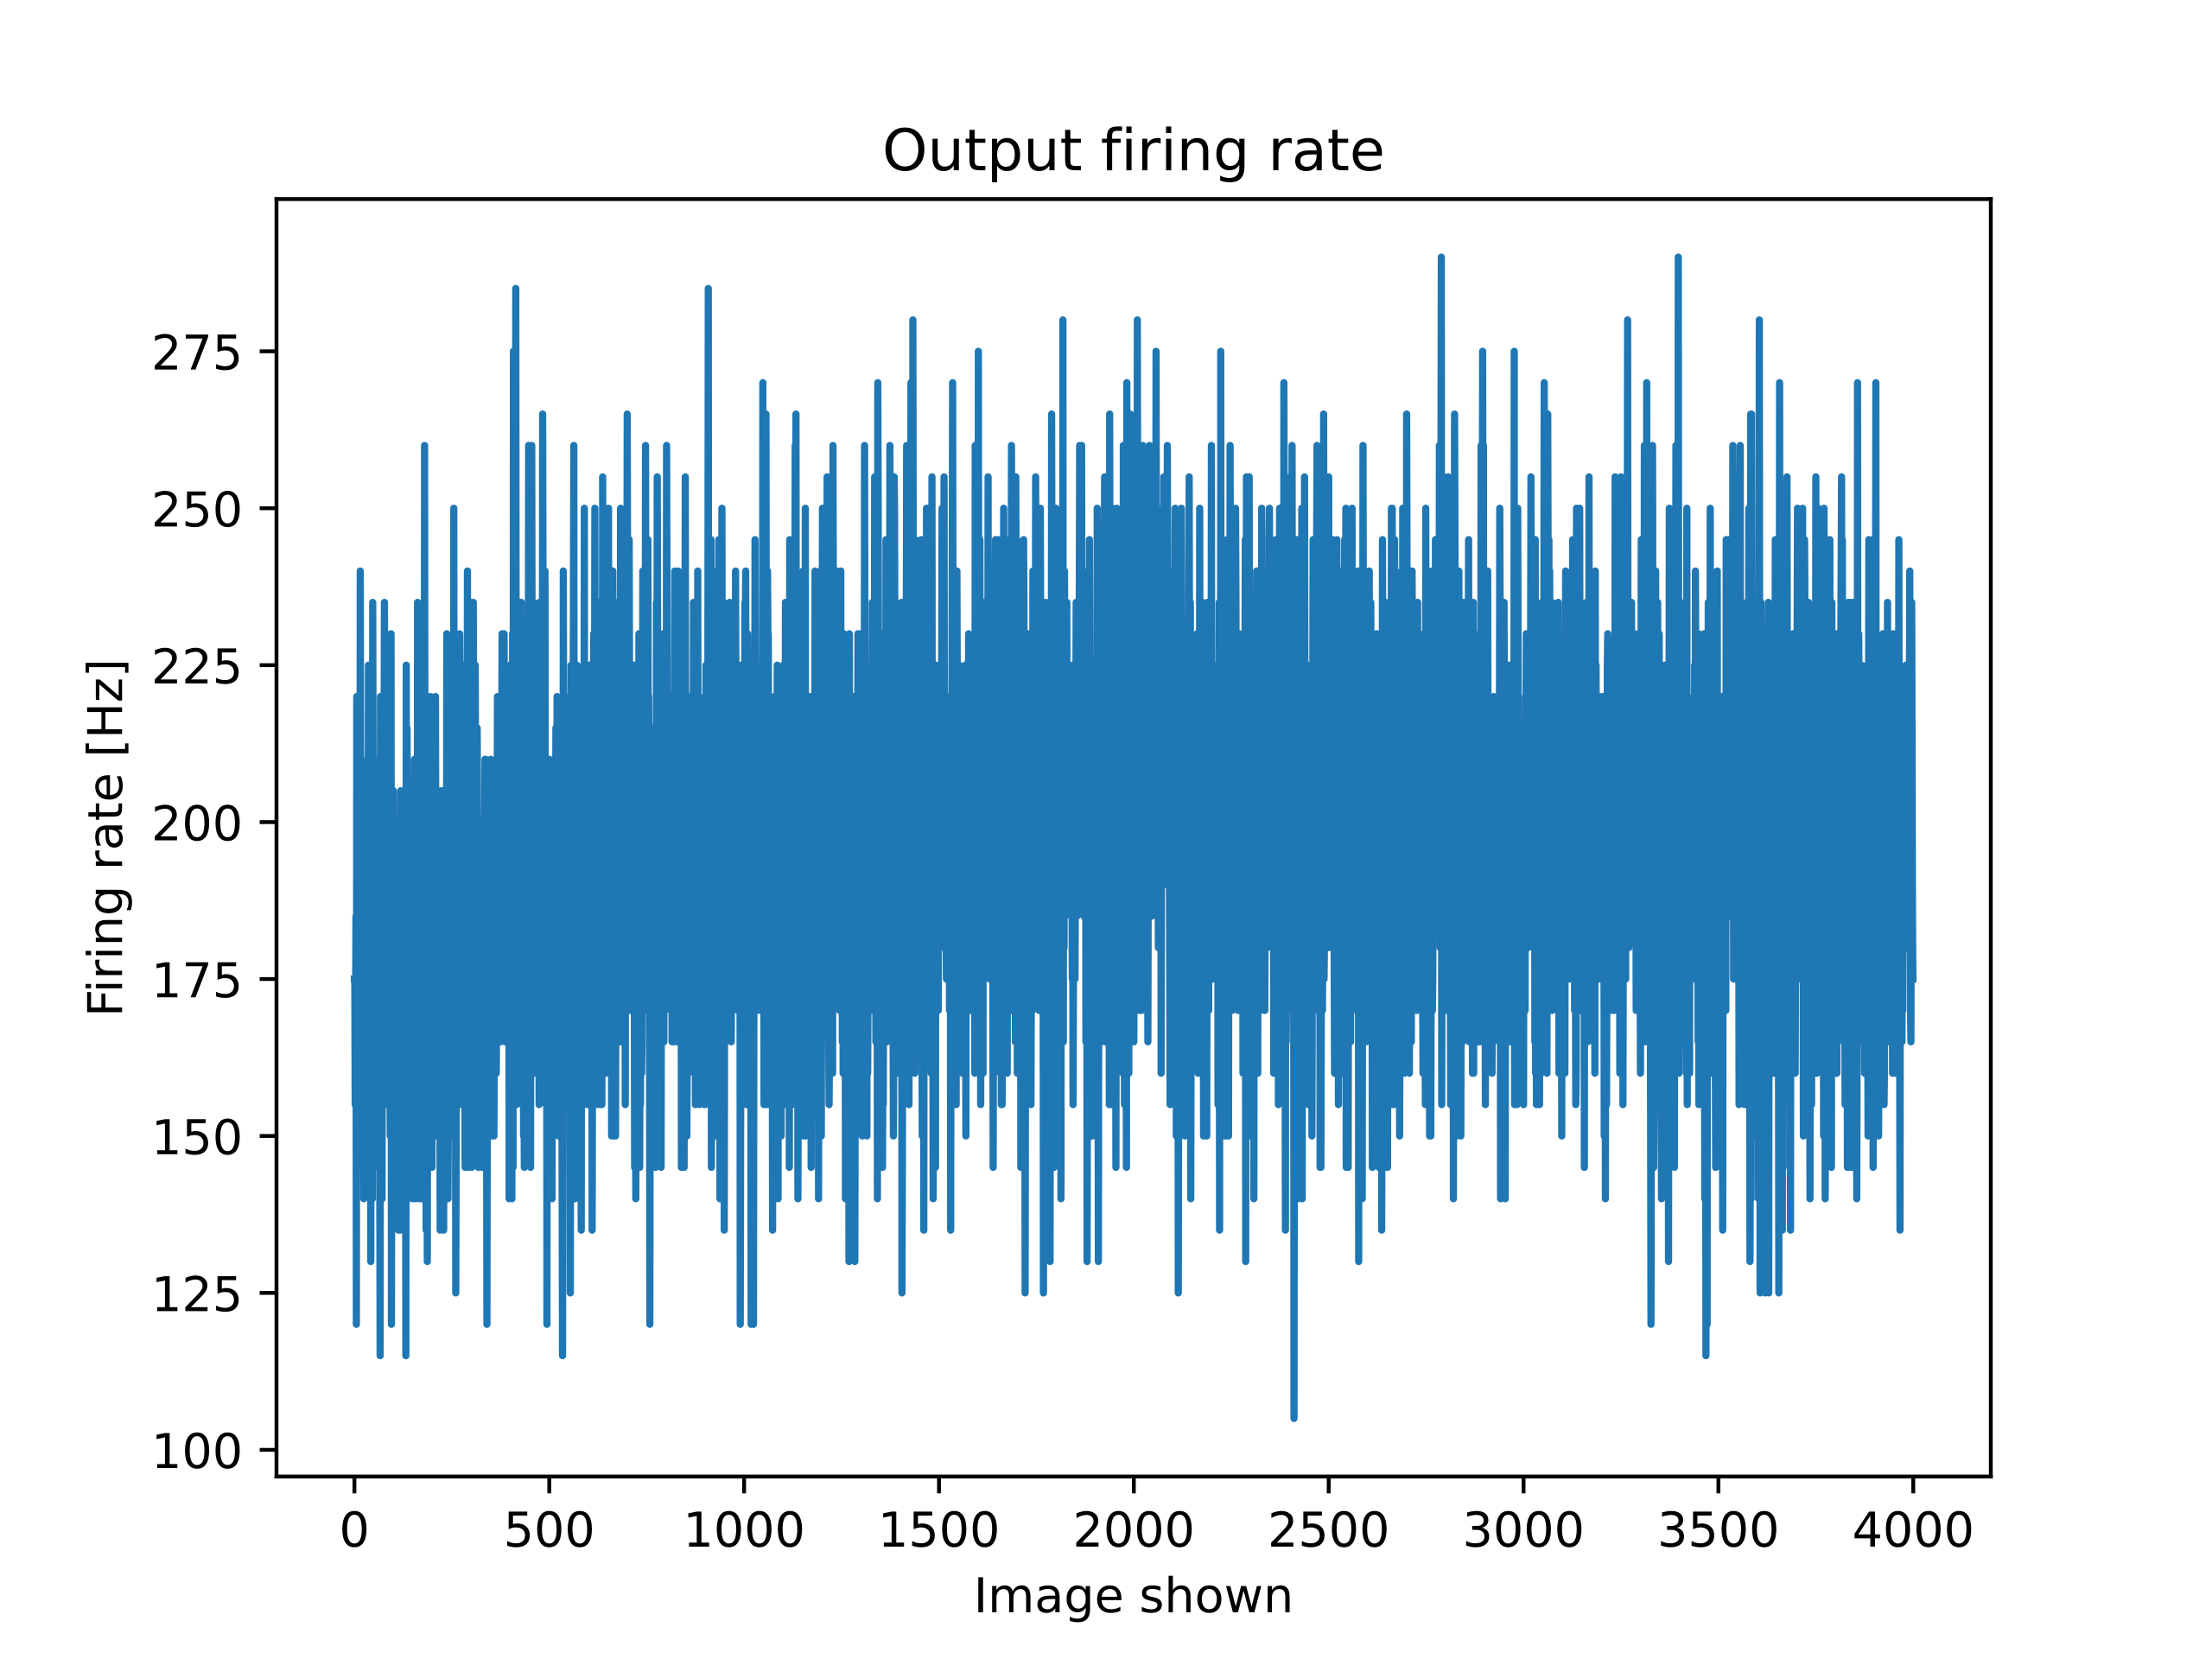
\includegraphics[width=\linewidth]{figures/angleAdaptiveInh/outputFiringRate.png}
  \caption{ Firing rate of all output neurons combined over the training process. }
  \label{fig:angleNetworkAdaptiveInhibitionOutputFiringRate}
\end{figure}

\begin{figure}
  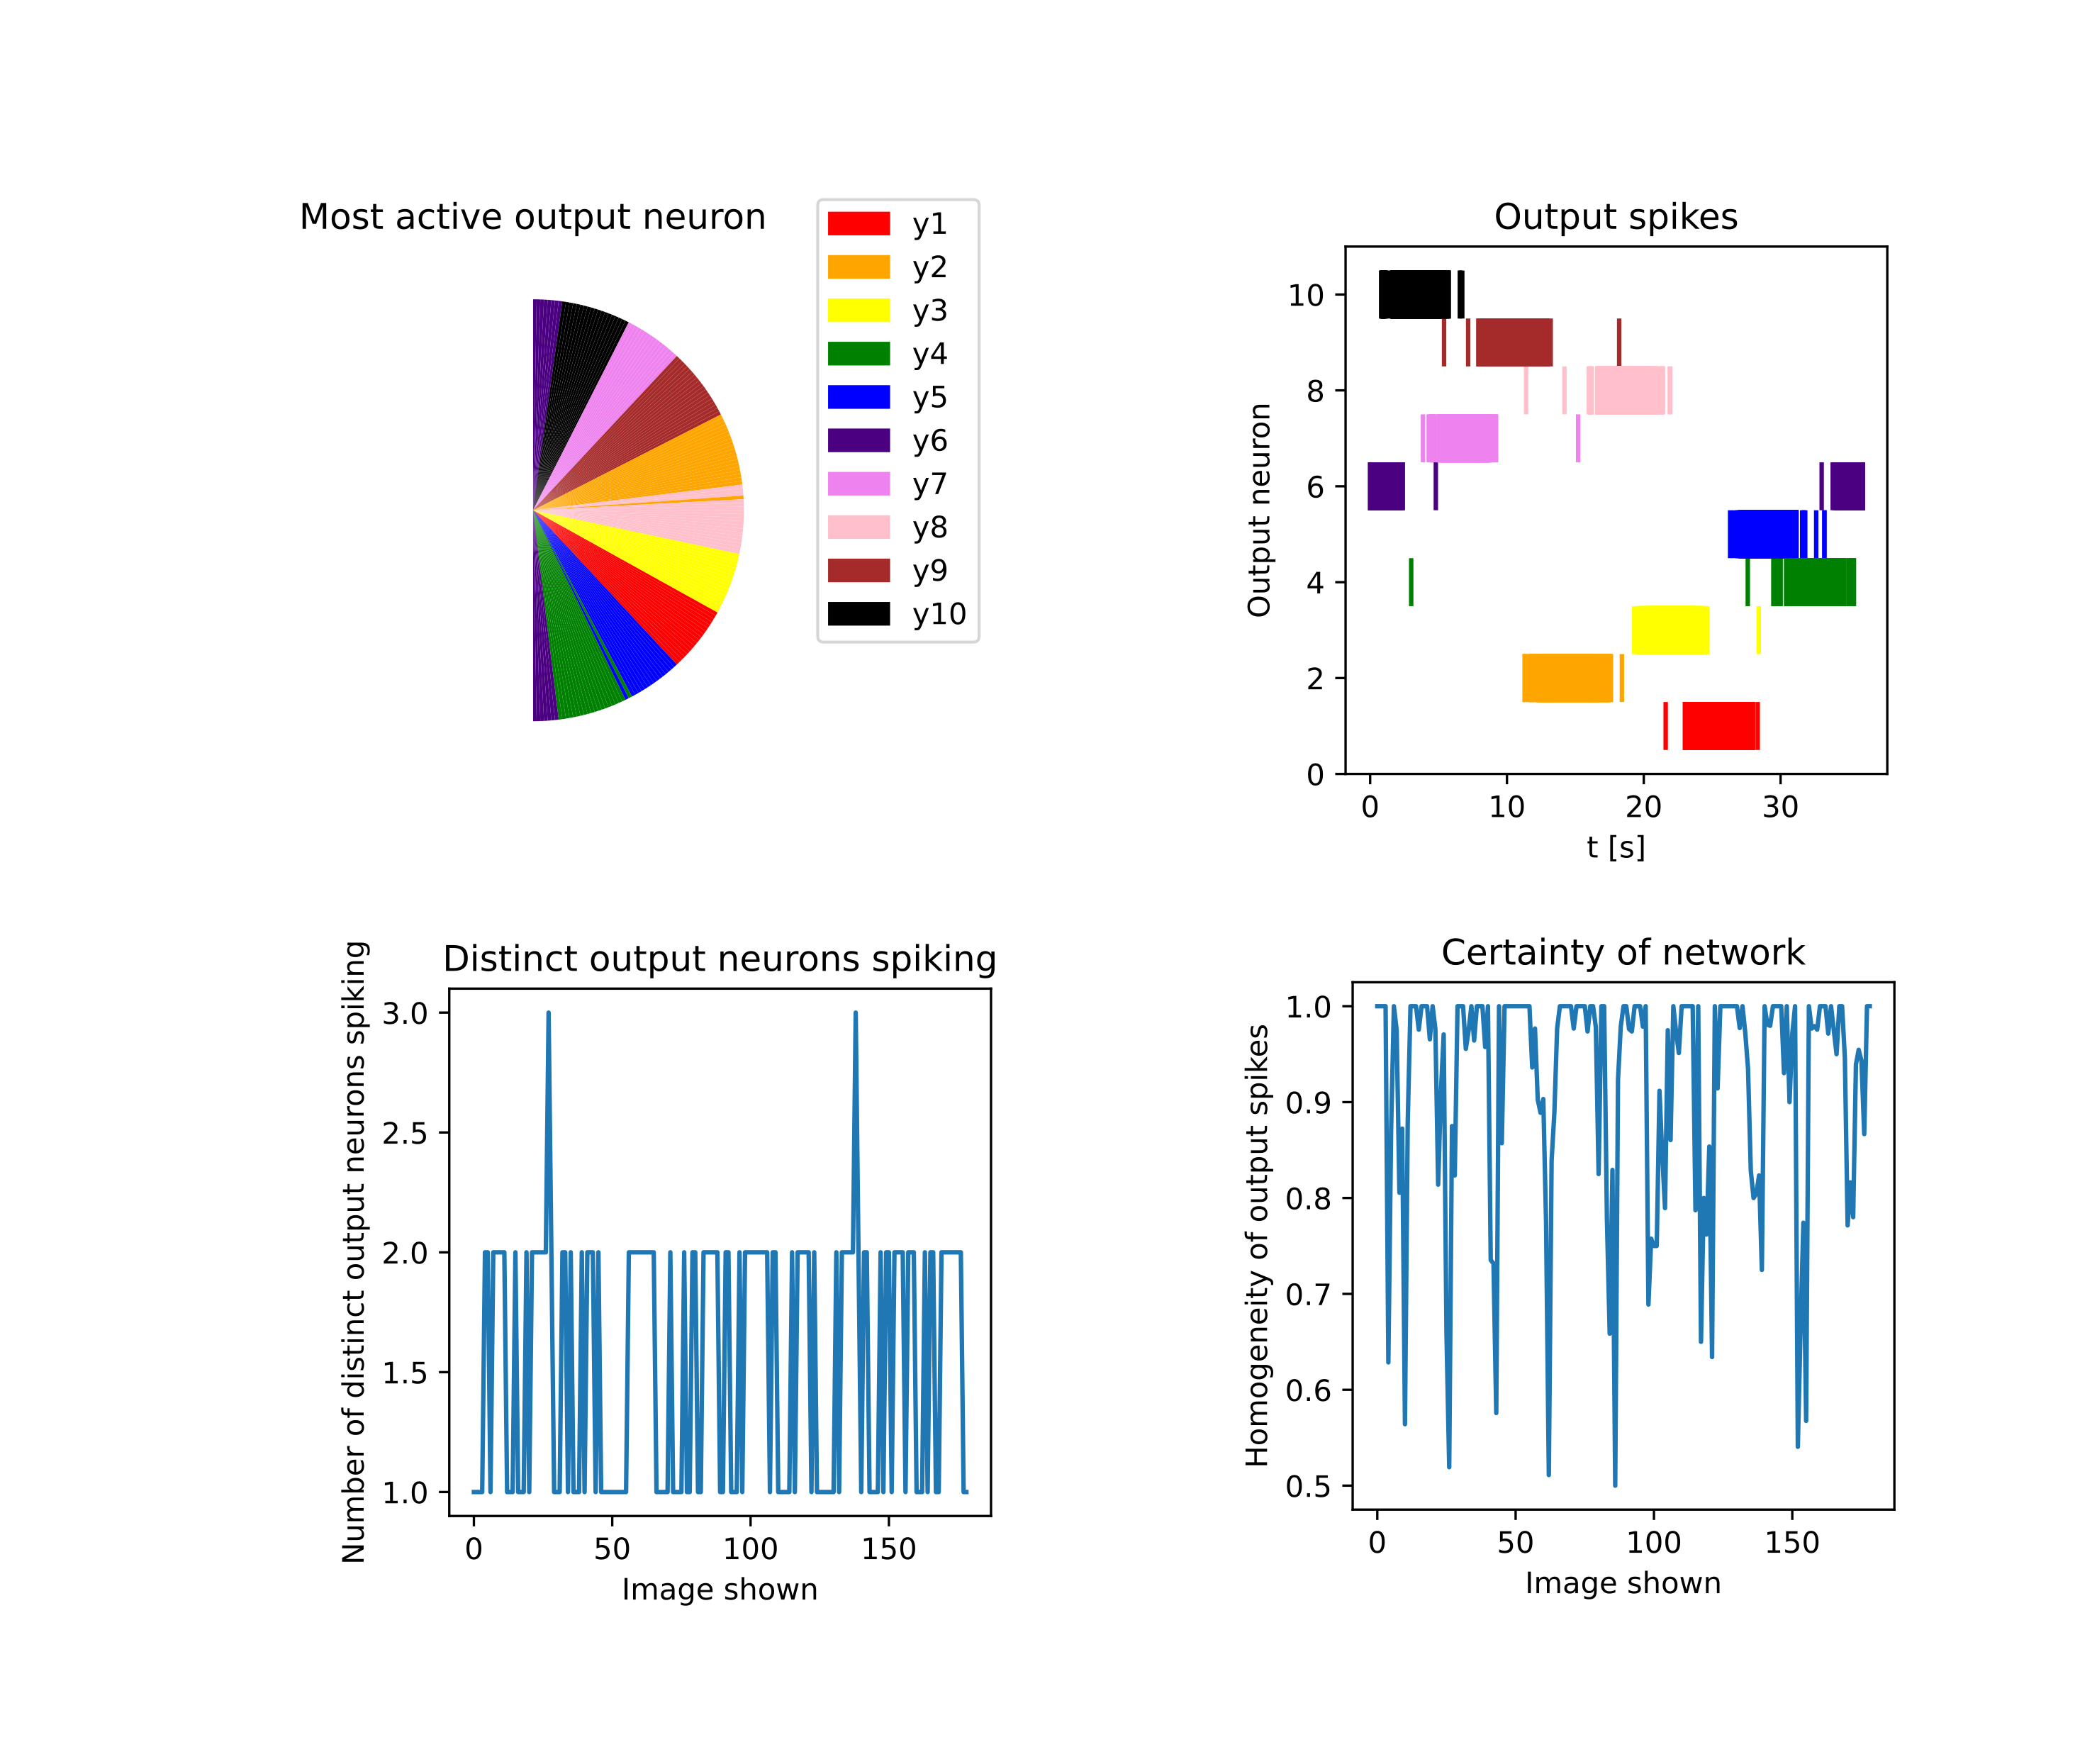
\includegraphics[width=\linewidth]{figures/angleAdaptiveInh/validation.png}
  \caption{\textbf{Validation.} \textbf{A} Most active output neuron depending on orientation of the training image. Training images were shown for 200 ms of each possible orientation in 1° steps. \textbf{B} Spike activity expressed by the output neurons during the validation process described in (\textbf{B}). \textbf{C} Number of distinct output neurons active during the presentation of each validation image. \textbf{D} Proportion (accuracy) of most active output neuron to activity of all other output neurons during the presentation duration of each training image.}
  \label{fig:angleNetworkAdaptiveInhibitionValidation}
\end{figure}

\section{Experiment 4: Rotated bars with adaptive inhibition}
\label{section:horvertAdaptiveInhibition}

\subsection{Introduction}

This experiment applies the adaptive inhibition already analysed in Experiment \ref{section:rotatedLinesAdaptiveInhibition} to Experiment \ref{section:horvert}. In Experiment \ref{section:horvert} the impact of the prior neurons was too small to influence the spiking activity of the output neurons. The newly implemented adaptive inhibition simplifies the process of changing the prior neurons, as it keeps the output firing frequency constant, thus preventing the need to perform a new parameter search upon each change to the prior neurons.

\subsection{Methods}

As in Experiment \ref{section:rotatedLinesAdaptiveInhibition} the firing rate of the output neurons was set to 200 Hz. To increase the influence of the prior neurons the firing rate of the prior neurons was increased from  50 Hz to 200 Hz. This change alone this not increase the impact of the prior neurons enough to help the network correctly detect a "cross-bar image" as either horizontal or vertical. It was also tried to increase the parameter $c_{prior}$ for the learning of the prior weights to shift the weight values towards bigger values. This did not increase the values of the weights, they stayed at a maximum of four. Thus the number of prior neurons had to be increased. Via grid search different numbers of prior neurons were tried.

\subsection{Results}

The tried parameters were as follows:
\begin{itemize}
  \item $c = c_{prior} = 20$
  \item $\lambda = 10^{-3}$
  \item number of prior neurons $ = 10, 20, 50, 100, 200$
\end{itemize}

For 50, 100 and 200 prior neurons the training process was impaired by the activity of the prior neurons. This arose as some output neurons responding to too large areas, while other prior neurons not responding to any specific areas. For 50 prior neurons four output neurons responded to horizontal bars, while six output neurons responded to vertical bars. This was unexpected and might be due to the stochastic nature of the training image generation. This was not yet analysed further and the validation of the network was performed with 20 prior neurons, as it was the largest amount of prior neurons that resulted in a properly trained network. The results of the training process can be seen in Figures \ref{fig:horvertAdaptiveInhibitionTraining} and \ref{fig:horvertAdaptiveInhibitionpriorWeights}.

\begin{figure}
  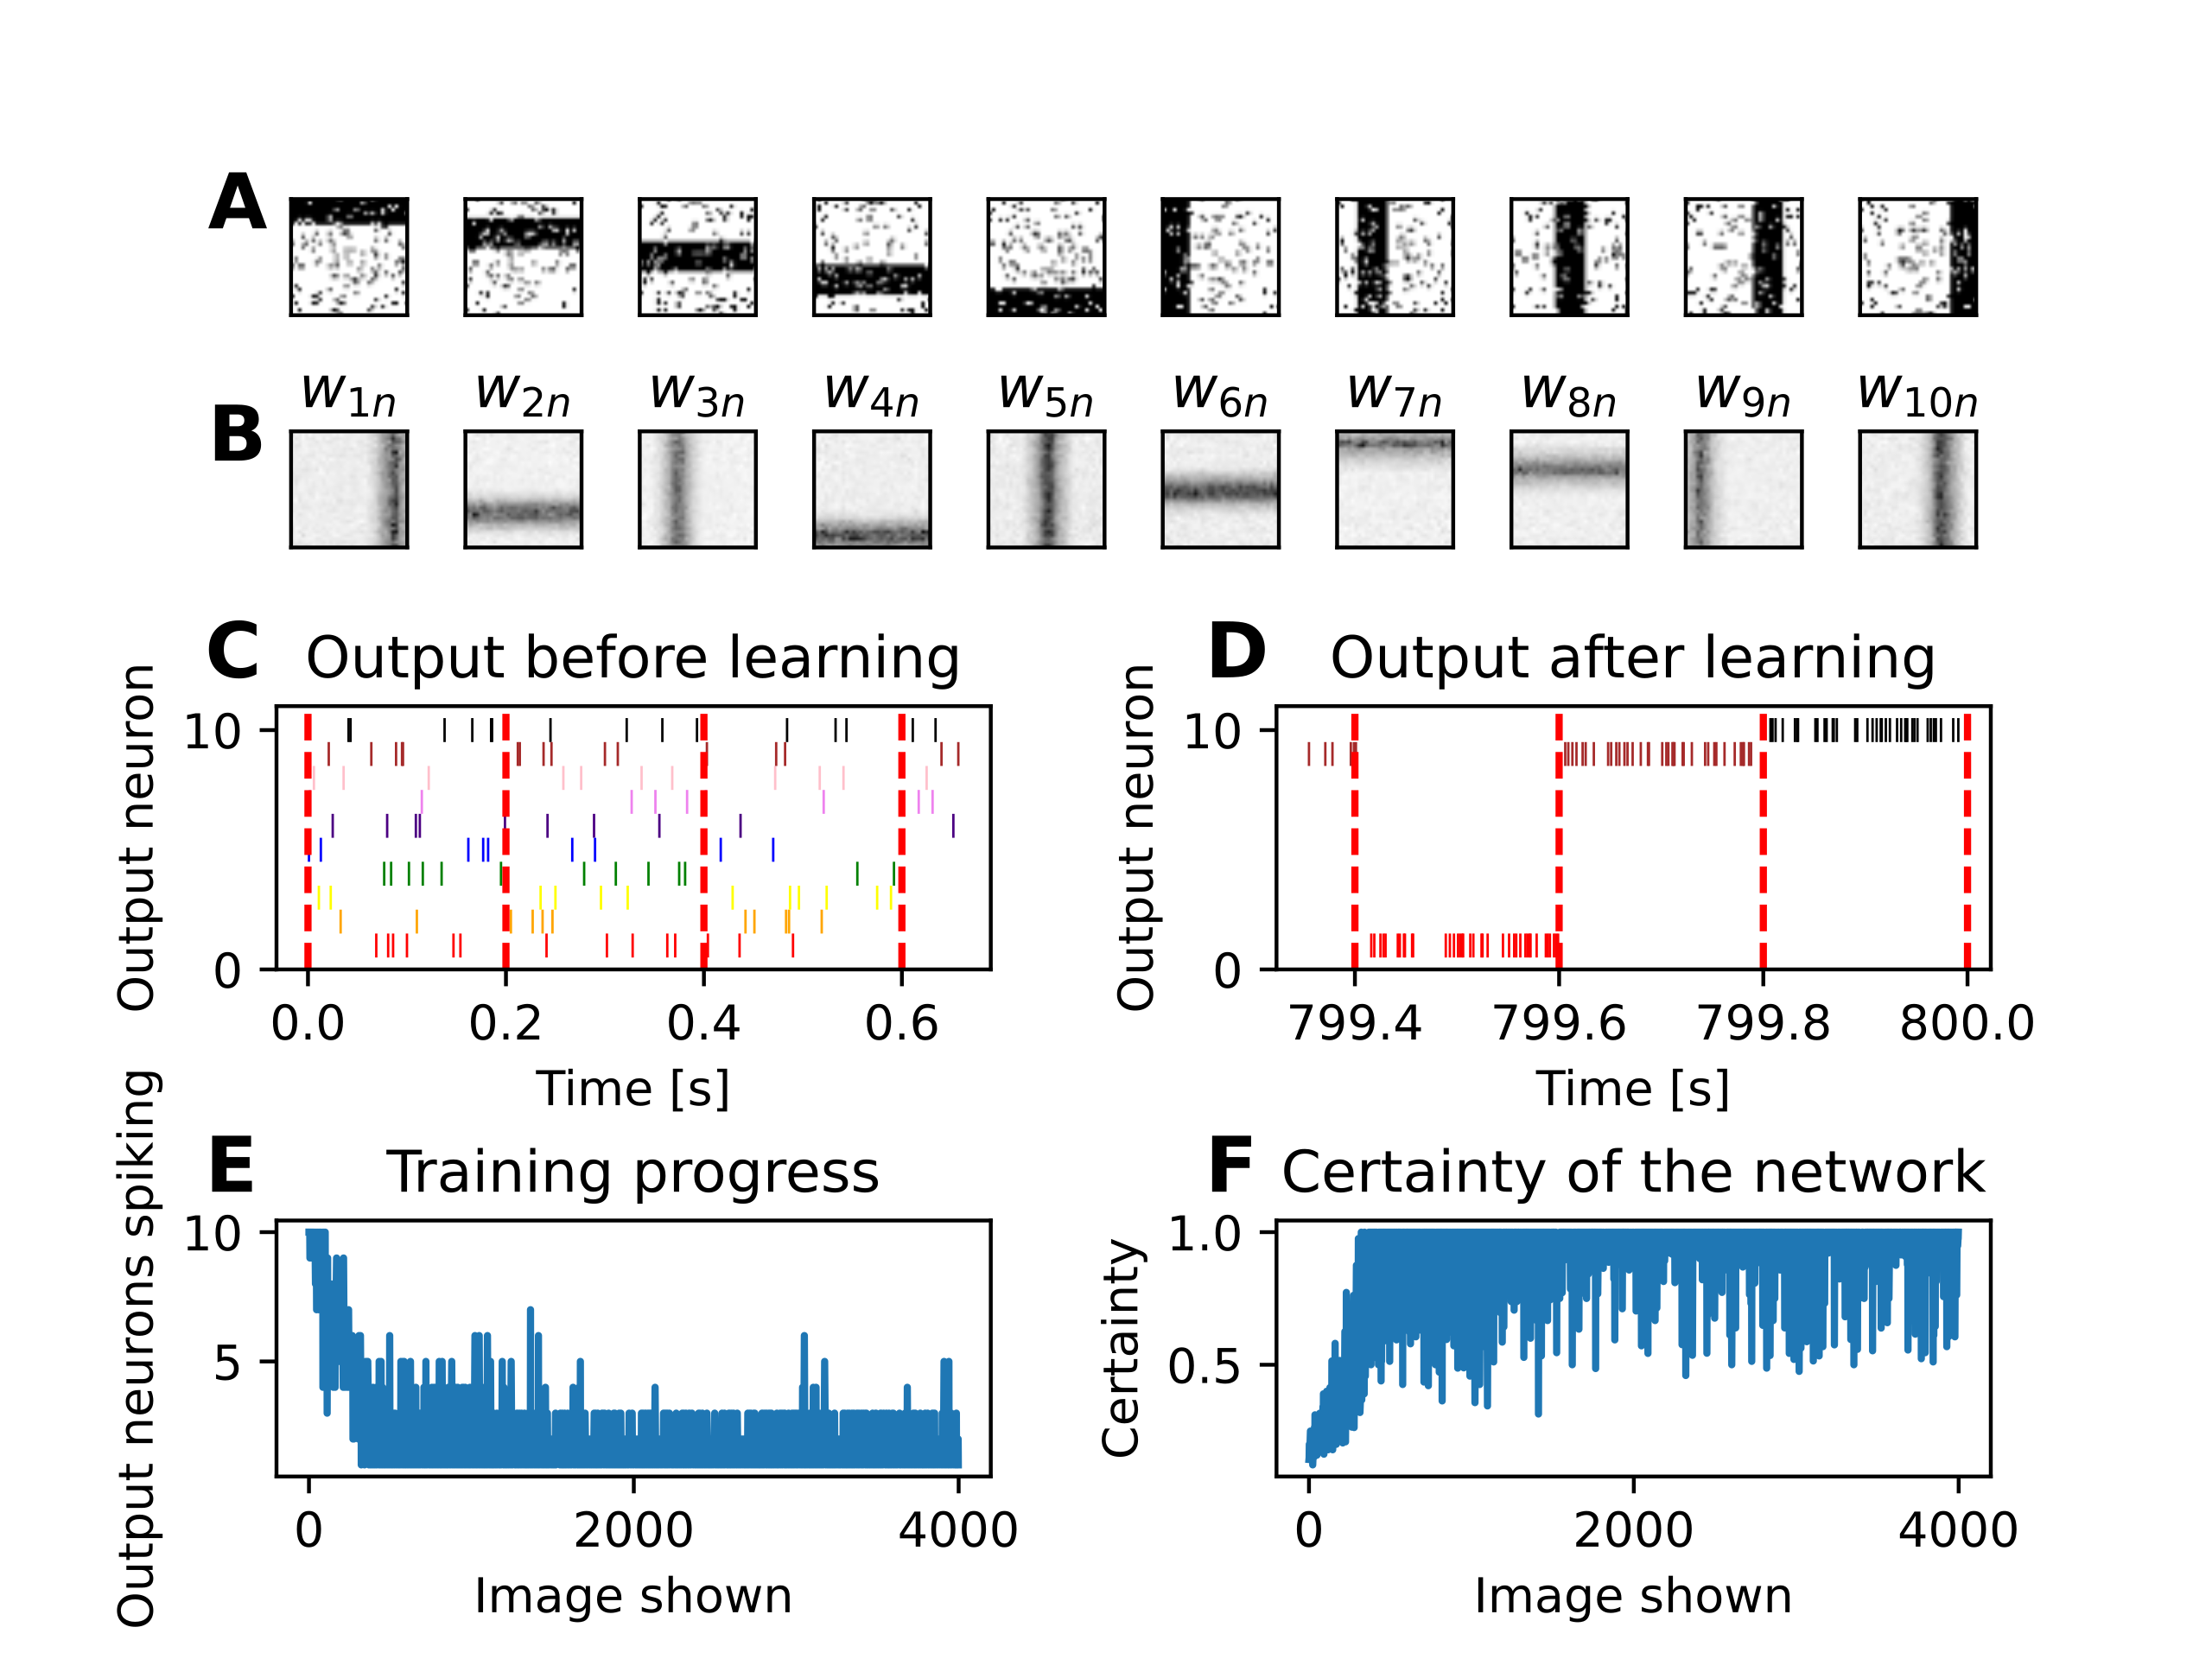
\includegraphics[width=\linewidth]{figures/horvertAdaptiveInh/trainingPlot.png}
  \caption{\textbf{Training with 20 prior neurons.} \textbf{A} Examples of 35 x 35-pixel input images of horizontal and vertical bars with background noise. \textbf{B} Learned weights of the connections between input and output neurons. \textbf{C, D} Spike activity expressed by the output neurons before and after the training of the network. \textbf{E} Number of distinct output neurons active during the presentation duration of each training image. \textbf{F} Proportion of most active output neuron  to activity of all other output neurons during the presentation duration of each training image.}
  \label{fig:horvertAdaptiveInhibitionTraining}
\end{figure}

\begin{figure}
  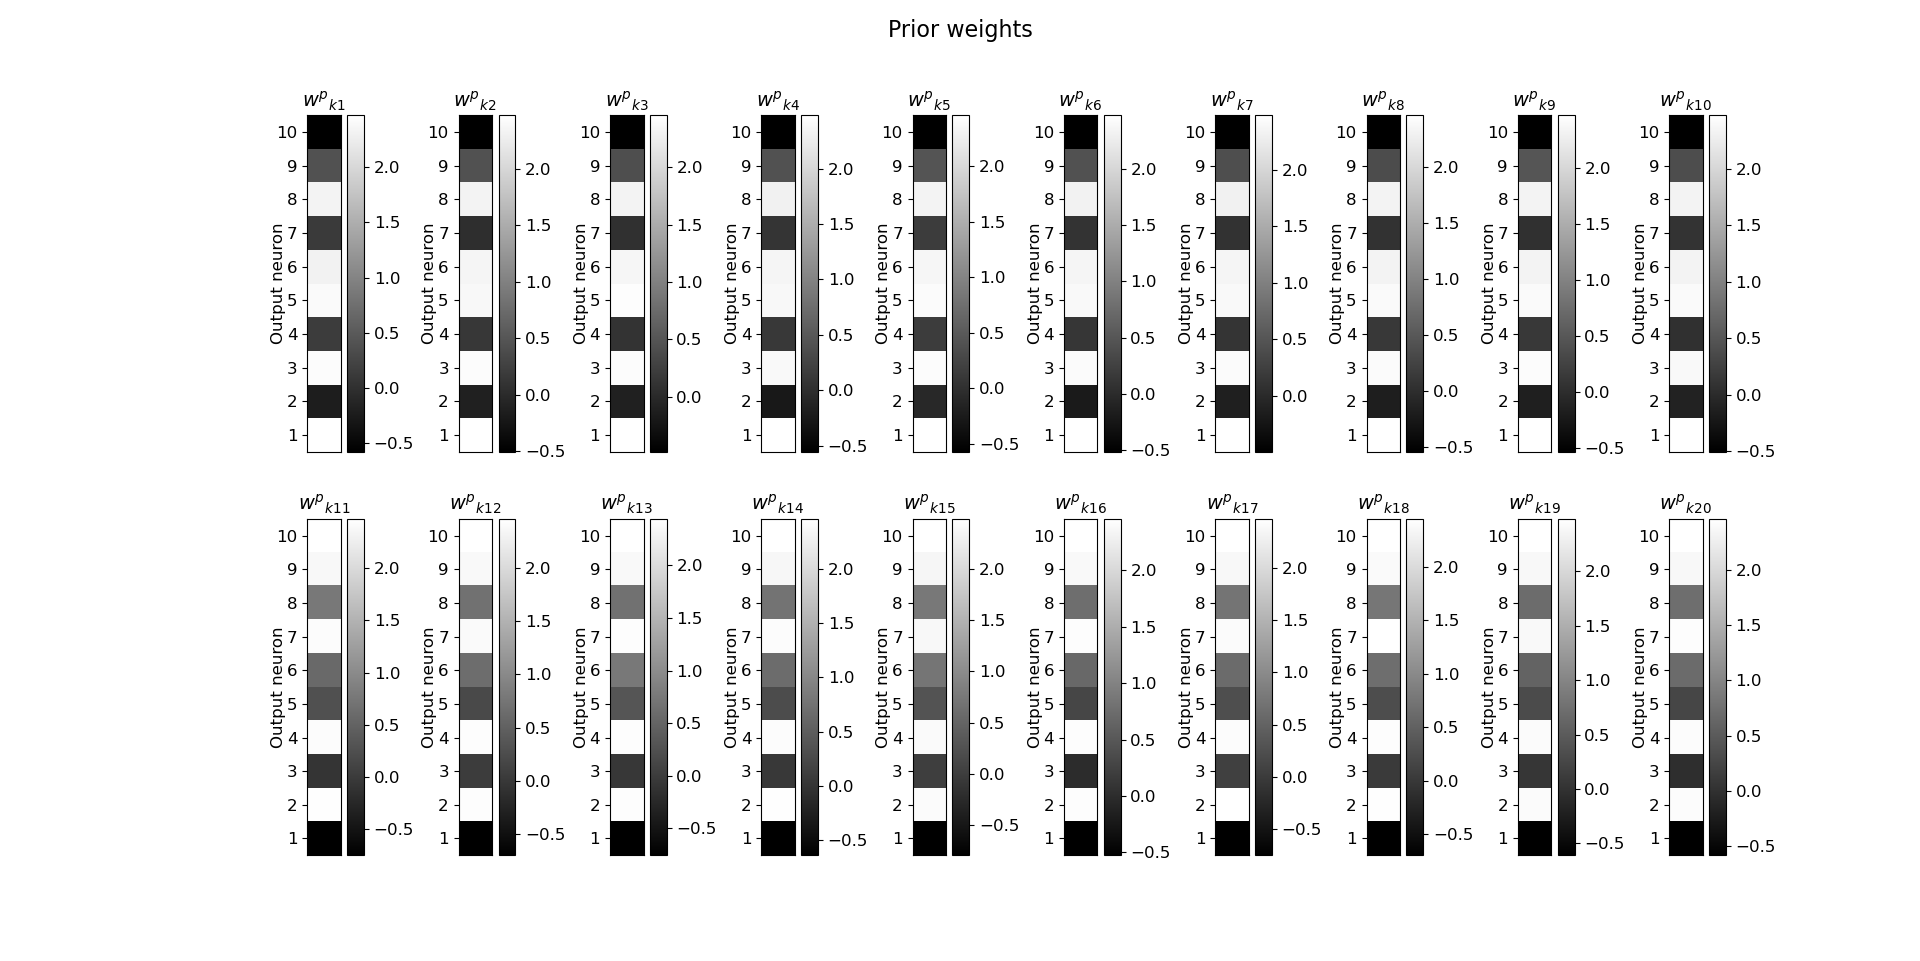
\includegraphics[width=\linewidth]{figures/horvertAdaptiveInh/priorWeights.png}
  \caption{ Learned weights of the connections between prior and output neurons. }
  \label{fig:horvertAdaptiveInhibitionpriorWeights}
\end{figure}

Next the impact of the prior was checked. To do this an image with one horizontal (at pixel 12) and one vertical bar (at pixel 5) on it was generated. Then the prior was set once to 0 (vertical) and once to 1 (horizontal). The image and the prior was then fed to the network. The cross image can be seen in Figure \ref{fig:horvertAdaptiveInhibitionPriorValImage}. The spiking activity depending on the prior can be seen in Figures \ref{fig:horvertAdaptiveInhibitionPriorValSpikes0} and \ref{fig:horvertAdaptiveInhibitionPriorValSpikes1}.

\begin{figure}
  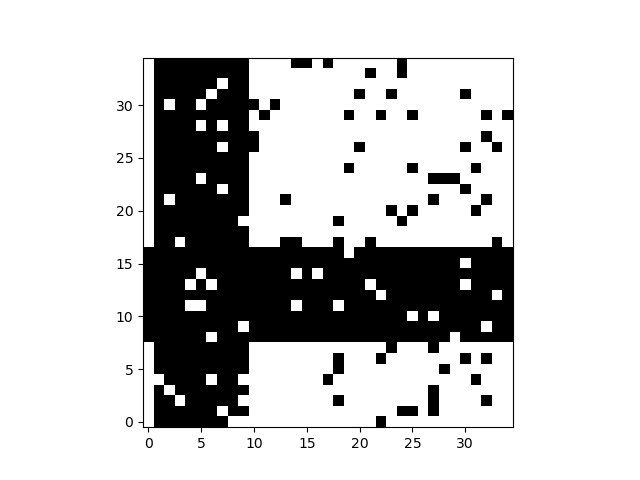
\includegraphics[width=\linewidth]{figures/horvertAdaptiveInh/20priors_pos5and12/crossImage.png}
  \caption{ Cross image fed to the network. }
  \label{fig:horvertAdaptiveInhibitionPriorValImage}
\end{figure}

\begin{figure}
  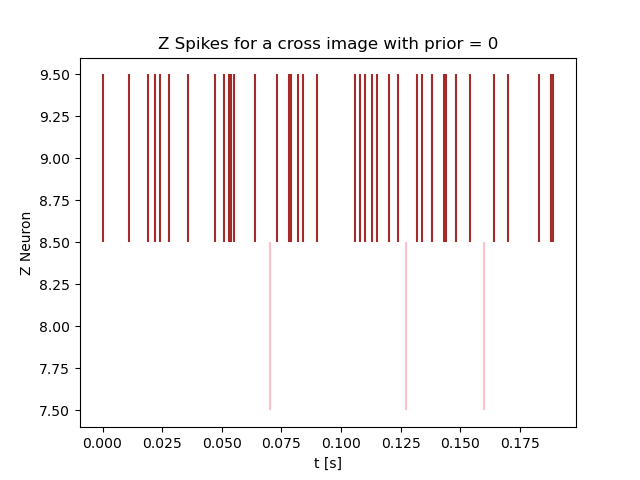
\includegraphics[width=\linewidth]{figures/horvertAdaptiveInh/20priors_pos5and12/crossZSpikes0.png}
  \caption{ Spiking activity of the output neurons with prior = 0. }
  \label{fig:horvertAdaptiveInhibitionPriorValSpikes0}
\end{figure}

\begin{figure}
  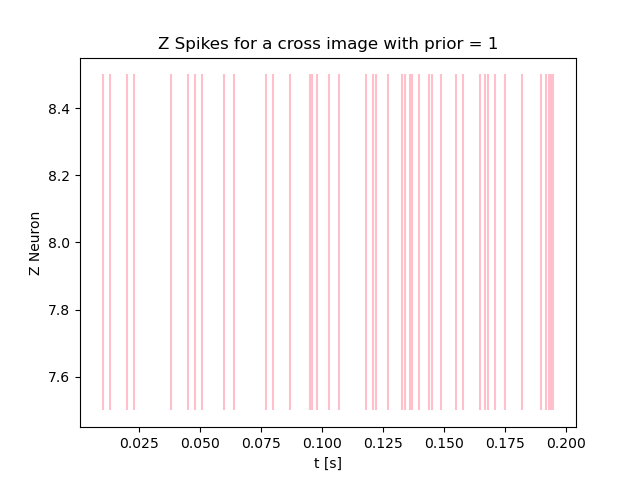
\includegraphics[width=\linewidth]{figures/horvertAdaptiveInh/20priors_pos5and12/crossZSpikes1.png}
  \caption{ Spiking activity of the output neurons with prior = 1. }
  \label{fig:horvertAdaptiveInhibitionPriorValSpikes1}
\end{figure}

To better show the impact of the prior it was gradually changed from horizontal to vertical. The starting firing frequency of the horizontal prior neurons was 200 Hz and 0 Hz for the vertical prior neurons. A cross image was shown to the network for 200 ms. After each image presentation duration the firing frequency of the horizontal prior neurons was decreased by 1 Hz and increased by 1 Hz for the vertical prior neurons. The used cross image can be seen in Figure \ref{fig:horvertAdaptiveInhibitionVariablePriorValImage}. The firing frequency of the 2 most active output neurons depending on the firing frequency of the vertical prior neurons can be seen in Figure \ref{fig:horvertAdaptiveInhibitionVariablePriorValFrequency}. As expected the correct horizontal output neuron is active in the beginning with about 200 Hz and the correct vertical output neuron is almost inactive. With rising firing frequency of the vertical prior neurons the activity of the horizontal output neurons decreases and the activity of the vertical output neurons increases. The membrane potentials of all output neurons for vertical prior neurons spiking with 200 Hz and horizontal prior neurons spiking with 0 Hz can be seen in Figure \ref{fig:horvertAdaptiveInhibitionVariablePriorValMembranePotentials}.

\begin{figure}
  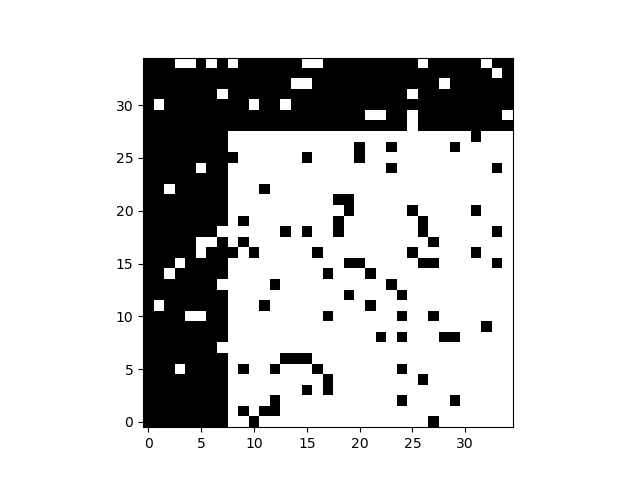
\includegraphics[width=\linewidth]{figures/horvertAdaptiveInh/crossImageForVariablePrior.png}
  \caption{ Cross image fed to the network. }
  \label{fig:horvertAdaptiveInhibitionVariablePriorValImage}
\end{figure}

\begin{figure}
  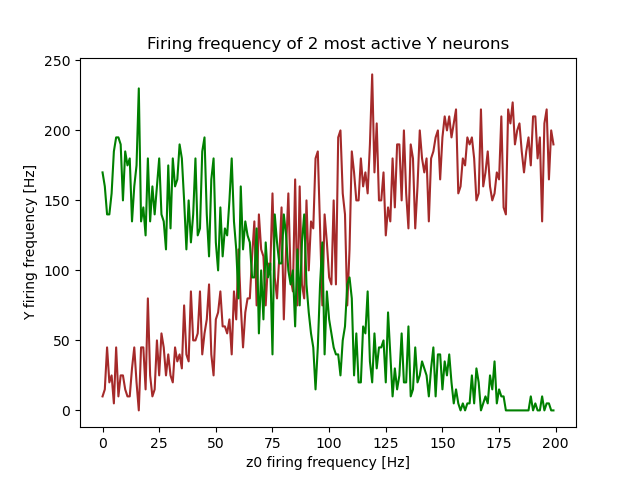
\includegraphics[width=\linewidth]{figures/horvertAdaptiveInh/YFrequency_prior199.png}
  \caption{ Firing frequency of the 2 most active output neurons depending on prior firing frequency. }
  \label{fig:horvertAdaptiveInhibitionVariablePriorValFrequency}
\end{figure}

\begin{figure}
  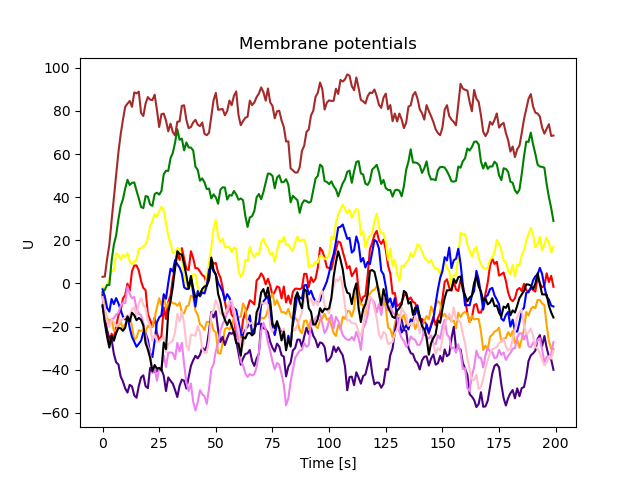
\includegraphics[width=\linewidth]{figures/horvertAdaptiveInh/membranePotentials0.png}
  \caption{ Membrane potentials of output neurons for vertical prior neurons spiking with 200 Hz and horizontal prior neurons spiking with 0 Hz. }
  \label{fig:horvertAdaptiveInhibitionVariablePriorValMembranePotentials}
\end{figure}


\section{Experiment 4: Mathematical analysis and simulation of a 1D network}
\label{section:1D}

\subsection{Introduction}

The purpose of this experiment was to mathematically analyse a simpler network, thus providing a definitive way to verify the performance of the simulation. The network was scaled down to be one-dimensional with 18 input neurons, four prior neurons and four output neurons, making it easier to analyse. The conditional probabilities of the input and output neurons of the network  were calculated by hand and then used to determine the theoretical posterior probability of the network. These probabilities were then used to calculate the weights for the simulation of the network. The distribution of the output spikes was then used to calculate the posterior probability of the simulation. The posterior probabilities of both the mathematical analysis and the simulation are compared, and by varying three parameters of the simulation it is tuned to approximate the analytical solution as closely as possible.

\subsection{Methods}

\paragraph{Network structure}
The architecture of this network remained the same as in previous experiments (with adaptive inhibition and a noise level of 10\%), only the amount of neurons was changed. The input image consists of nine pixels in a horizontal line. Within those nine pixels four output classes can be represented. Each output class consists of three pixels next to each other. This results in each output class overlapping its neighbour classes by one pixel. Thus the centres of the output classes are at position 1, 3, 5 and 7.    As there have to be 2 input neurons for each pixel, one neuron being active if the pixel is white and one if the pixel is black, the network has 18 input neurons. Furthermore four prior neurons were implemented, of which only one is being active for one of the output classes at a time. Lastly the network has four output neurons.

\paragraph{Mathematical Analysis}
The posterior probability of the network was calculated by using
\begin{equation}
\label{eqn:pYvorausgesetztXUndZ}
P(Y = i|X = x, Z = j) = \frac{P(X=x|Y=i)P(Y = i|Z = j)}{\Sigma_{k}P(X=x,Y=k)P(Y=k|Z=j)}.
\end{equation}
$P(X=x|Y=i)$ and $P(Y=i|Z=j)$ were derived by hand corresponding to the paradigm of the experiment. The calculation of $P(X=x|Y=i)$ was split into two parts. First the contribution of the active input neurons was calculated by determining the matrix $P^{X|Y}$. This matrix is of size 4 x 9 and contains the conditional probabilities of each input neuron $y_i$ being active, given that an output neuron $x_l$ is active. These probabilities were calculated by determining which input neurons are active depending on the output class and which input neurons are inactive, as dictated by the network structure.  Furthermore the noise that was applied to the input neurons had to be taken into account. For input neurons belonging to the output class the conditional probability was determined as 1 and lowered by the noise level, while for the input neurons outside of the 3-wide pixel block belonging to the output class it was determined as 0 and raised by the noise level. According to this algorithm $P^{X|Y}$ is given by
\begin{equation}
\label{eqn:PXvorausgesetztYIf}
P_{i,l}^{X|Y} = \begin{dcases*} 1 - $noise level$ & if $x_l$ is in the active area of $y_i$, \\
0 + $noise level$ & \text{if $x_l$ is not in the active area of $ y_i $ } \end{dcases*}.\end{equation}
  After calculating all entries of $P^{X|Y}$ its rows were multiplied with the input image vector
\begin{equation}
\label{eqn:p1XvorausgesetztYMalX}
P_1(X = x|Y = i) = P^{X|Y}_{i,*} \cdot x
\end{equation}
resulting in a conditional probability for each output class depending on the input vector. The input vector was given with entries of 1 for active pixels and with entries of 0 for inactive pixels.
Next to include the contribution of the input neurons that are spiking when a pixel is inactive the conditional probability of the input neurons that are active for the entries where $x_i = 0$ had to be calculated. To achieve this complementary conditional probability at first $P^{X|Y}$ was subtracted from one. To include the correct conditional probabilities for the complementary case the input image vector x was then also subtracted from one. $1 - P^{X|Y}$ and $1 - x$ were multiplied to yield
\begin{equation}
\label{eqn:p2minusXvorausgesetztYMalX}
P_2(X = x|Y = i) = (1 - P^{X|Y}_{i,*}) \cdot (1 - x).
\end{equation}
The results of both calculations were then multiplied element-wise to yield
\begin{equation}
\label{eqn:pXvorausgesetztY}
P(X = x|Y = i) = P_1(X = x|Y = i) \odot P_2(X = x|Y = i).
\end{equation}
$P(Y=i|Z=j)$ was determined by first calculating the matrix $P^{Y|Z}$. It has a dimension of 4 x 4 and contains the conditional probabilities for the output neuron $y_i$, given the prior neuron $z_j$ being active. For each output class there exists one corresponding prior neuron. As there can never be more than one active prior neuron at a time $P^{Y|Z}$ is given by
\begin{equation}
\label{eqn:PYvorausgesetztZIf}
P_{j,i}^{Y|Z} = \begin{dcases*} 1 - $noise level$ & if $i = j$, \\
0 +  \frac{1}{3}  $noise level$ & \text{if $i \neq j$. } \end{dcases*}\end{equation} 
$P(Y=i|Z=j)$ was then obtained by
\begin{equation}
\label{eqn:pYvorausgesetztZ}
P(Y=i|Z=j) = P^{Y|Z} \cdot z
\end{equation}
where z is given by a 4 x 1 one-hot encoded vector of the prior.

\paragraph{Simulation}
The input weights for the simulation were calculated as two separate sets. First weights $w_1$ for the input neurons that are active for active input pixels were determined by 
\begin{equation}
\label{eqn:1DWeights}
w_1 = \ln(P^{X|Y}).
\end{equation}
Second complementary input weights $w_2$ were calculated for  input neurons representing non active input pixels with
\begin{equation}
\label{eqn:1DWeightsComplementary}
w_2 = \ln(1 - P^{X|Y}).
\end{equation} 
The prior weights $w_p$ were derived by 
\begin{equation}
\label{eqn:1DWeightsPrior}
w_p = \ln(P^{Y|Z}).
\end{equation}
The network was simulated for six different input images for each parameter set. After the image presentation period of each input image the amount of the output spikes of different classes were counted and their proportions were calculated to yield the "simulation output probabilities" in later plots. The Kullback-Leibler divergence was chosen to compare the divergence of the analytic and the simulated results of the network. This metric indicates how much two probability distributions diverge from each other. The goal of the parameter search of the simulation was to minimize the Kullback-Leibler divergence. Upon completion of the simulation of an output image the Kullback-Leibler divergence was calculated for that image
\begin{equation}
\begin{split}
\label{eqn:KLDivergence}
D_{KL}(P_{analysis}(Y = i|X, Z)||P_{simulation}(Y = i|X, Z)) = \\ \sum_{i=1}^K P_{analysis}(Y = i|X, Z) \cdot \ln( \frac{P_{analysis}(Y = i|X, Z)}{P_{simulation}(Y = i|X, Z)})
\end{split}
\end{equation}
where K is the number of output neurons and $P_{analysis}(Y = i|X, Z)$ and $P_{simulation}(Y = i|X, Z)$ are the "analysis output probabilities" and "simulation output probabilities". The six resulting Kullback-Leibler divergences for each parameter set were then averaged to create a single metric by which the performance of the different parameter sets was compared. The three parameters input firing rate $f_{input}$, prior firing rate $f_{prior}$ and the membrane constant $\tau_{decay}$ were varied to inspect their influence on the result, as well as to approximate the analytical solution as closely as possible. Each input image is presented to the network for 20 seconds to reduce the variance between runs. Furthermore each simulation was repeated 20 times with the same parameter set to obtain the mean and standard deviation of the simulation output probabilities and of the Kullback-Leibler divergence.

\subsection{Results}

\paragraph{Analytic Results}

First the matrix $P^{X|Y}$ was analytically calculated by using Equation \ref{eqn:PXvorausgesetztYIf} 
\begin{equation}
\label{eqn:pXvorausgesetztYResult}
P^{X|Y} = \begin{bmatrix}
0.9 & 0.9 & 0.9 & 0.1 & 0.1 & 0.1 & 0.1 & 0.1 & 0.1\\
0.1 & 0.1 & 0.9 & 0.9 & 0.9 & 0.1 & 0.1 & 0.1 & 0.1\\
0.1 & 0.1 & 0.1 & 0.1 & 0.9 & 0.9 & 0.9 & 0.1 & 0.1\\
0.1 & 0.1 & 0.1 & 0.1 & 0.1 & 0.1 & 0.9 & 0.9 & 0.9\\
\end{bmatrix}.
\end{equation}
Next the matrix $P^{Y|Z}$ was analytically calculated by using Equation \ref{eqn:PYvorausgesetztZIf} 
\begin{equation}
\label{eqn:pYvorausgesetztZResult}
P^{Y|Z} = \begin{bmatrix}
0.9 & 0.0333 & 0.0333 & 0.0333\\
0.0333 & 0.9 & 0.0333 & 0.0333\\
0.0333 & 0.0333 & 0.9 & 0.0333\\
0.0333 & 0.0333 & 0.0333 & 0.9\\
\end{bmatrix}.
\end{equation} 
For each input image these two matrices were then  multiplied with the input vector and prior vector as described Equations \ref{eqn:p1XvorausgesetztYMalX}, \ref{eqn:p2minusXvorausgesetztYMalX},  \ref{eqn:pXvorausgesetztY} and \ref{eqn:pYvorausgesetztZ} to yield $P(X = x|Y = i)$ and $P(Y=i|Z=j)$. Using  \ref{eqn:pYvorausgesetztXUndZ} then 
yielded $P(Y = i|X = x, Z = j)$ also called "Analysis output probabilities" in later plots.

\paragraph{Simulation results without prior}
To simplify the parameter fitting process the network was at first simulated with inactive prior neurons. Only after determining the best values for $f_{input}$ and $\tau_{decay}$ were the prior neurons reactivated and $f_{prior}$ was fitted. The values 0.015 seconds and 0.004 seconds for $\tau_{decay}$ were used for the simulation and compared. For each of these values an optimal value for $f_{input}$ was found by simulating different values and looking for the value that yields the smallest Kullback-Leibler divergence.

\subparagraph{$\tau_{decay} = 0.015 seconds$, $f_{prior} = 0 Hz$}
Values for $f_{input}$ between 10 and 110 Hz in steps of 10 Hz were simulated. After identifying the input firing rate with the smallest Kullback-Leibler divergence the network was simulated again for $f_{input}$ values $\pm$ 10 Hz in steps of 2 Hz of the best value. This process yielded the best input firing rate of 42 Hz. The results of this parameter combination can be seen in Figure \ref{fig:1D_42_0_15}. In this figure six different input images can be seen marked with the letter "A". The active pixels are shown in black.  The posterior probability of the mathematical analysis can be seen next to the letter "B". And finally the proportion of output spikes of the different output neurons can be seen next to the letter "C". Each probability of "C" has a standard deviation next to it, which was calculated over 20 runs of the network. At the bottom the value of the Kullback-Leibler divergence is given, with its standard deviation next to it.

\begin{figure}
  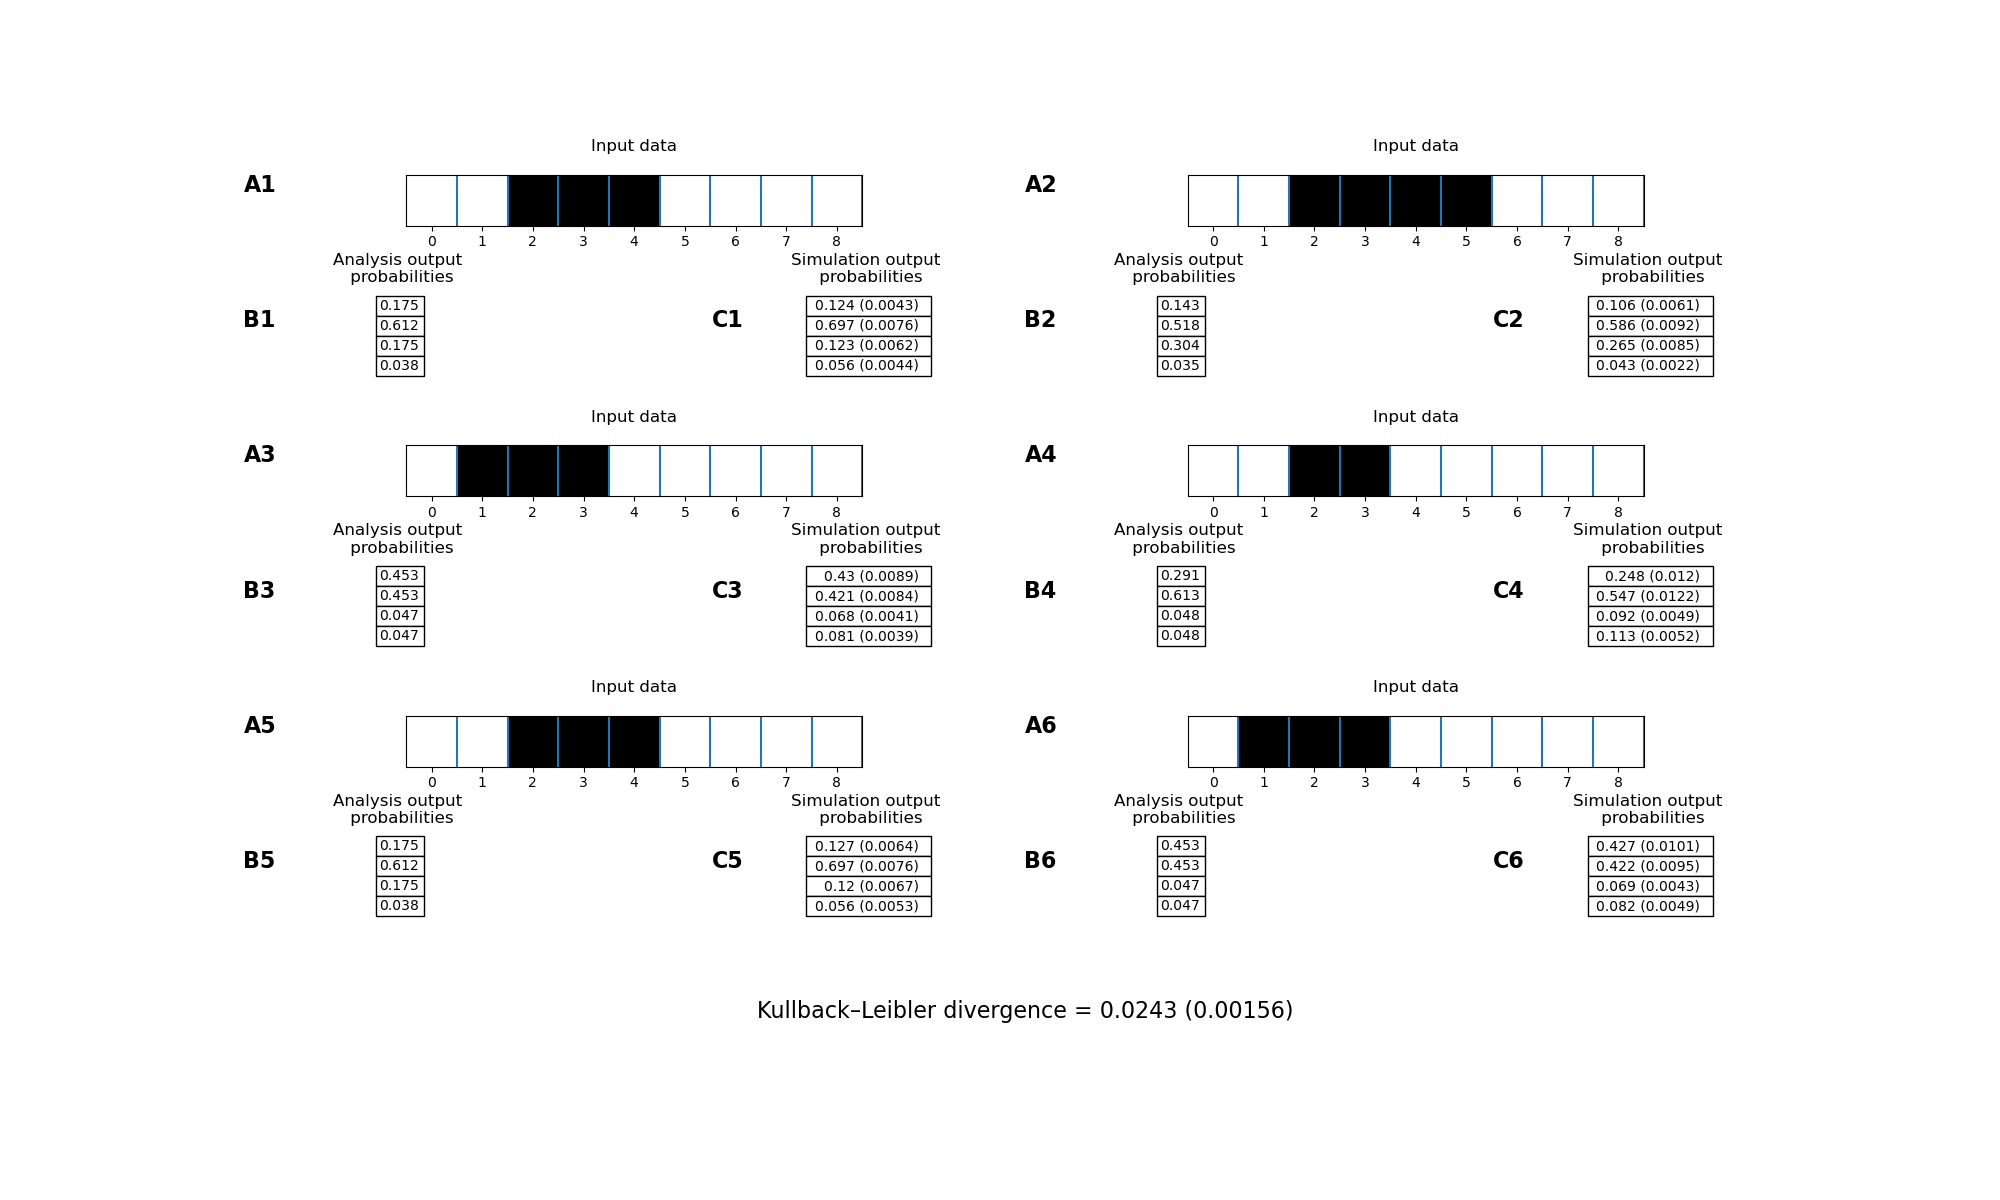
\includegraphics[width=\linewidth]{figures/1D/1D_42_0_15.png}
  \caption{\textbf{Analysis and simulation result. Parameters: } $f_{input} = 42 Hz, f_{prior} = 0 Hz, \tau_{decay} = 15 ms$ \textbf{A} Input images with 9 x 1 pixels. \textbf{B} Analytically calculated posterior probabilities. \textbf{C} Proportions of the spikes of the output neurons during the simulation and their standard deviations in brackets.}
  \label{fig:1D_42_0_15}
\end{figure}

When $f_{input}$ was 70 Hz the results of the analysis and the simulation differed more as can be seen in Figure \ref{fig:1D_70_0_15}.

\begin{figure}
  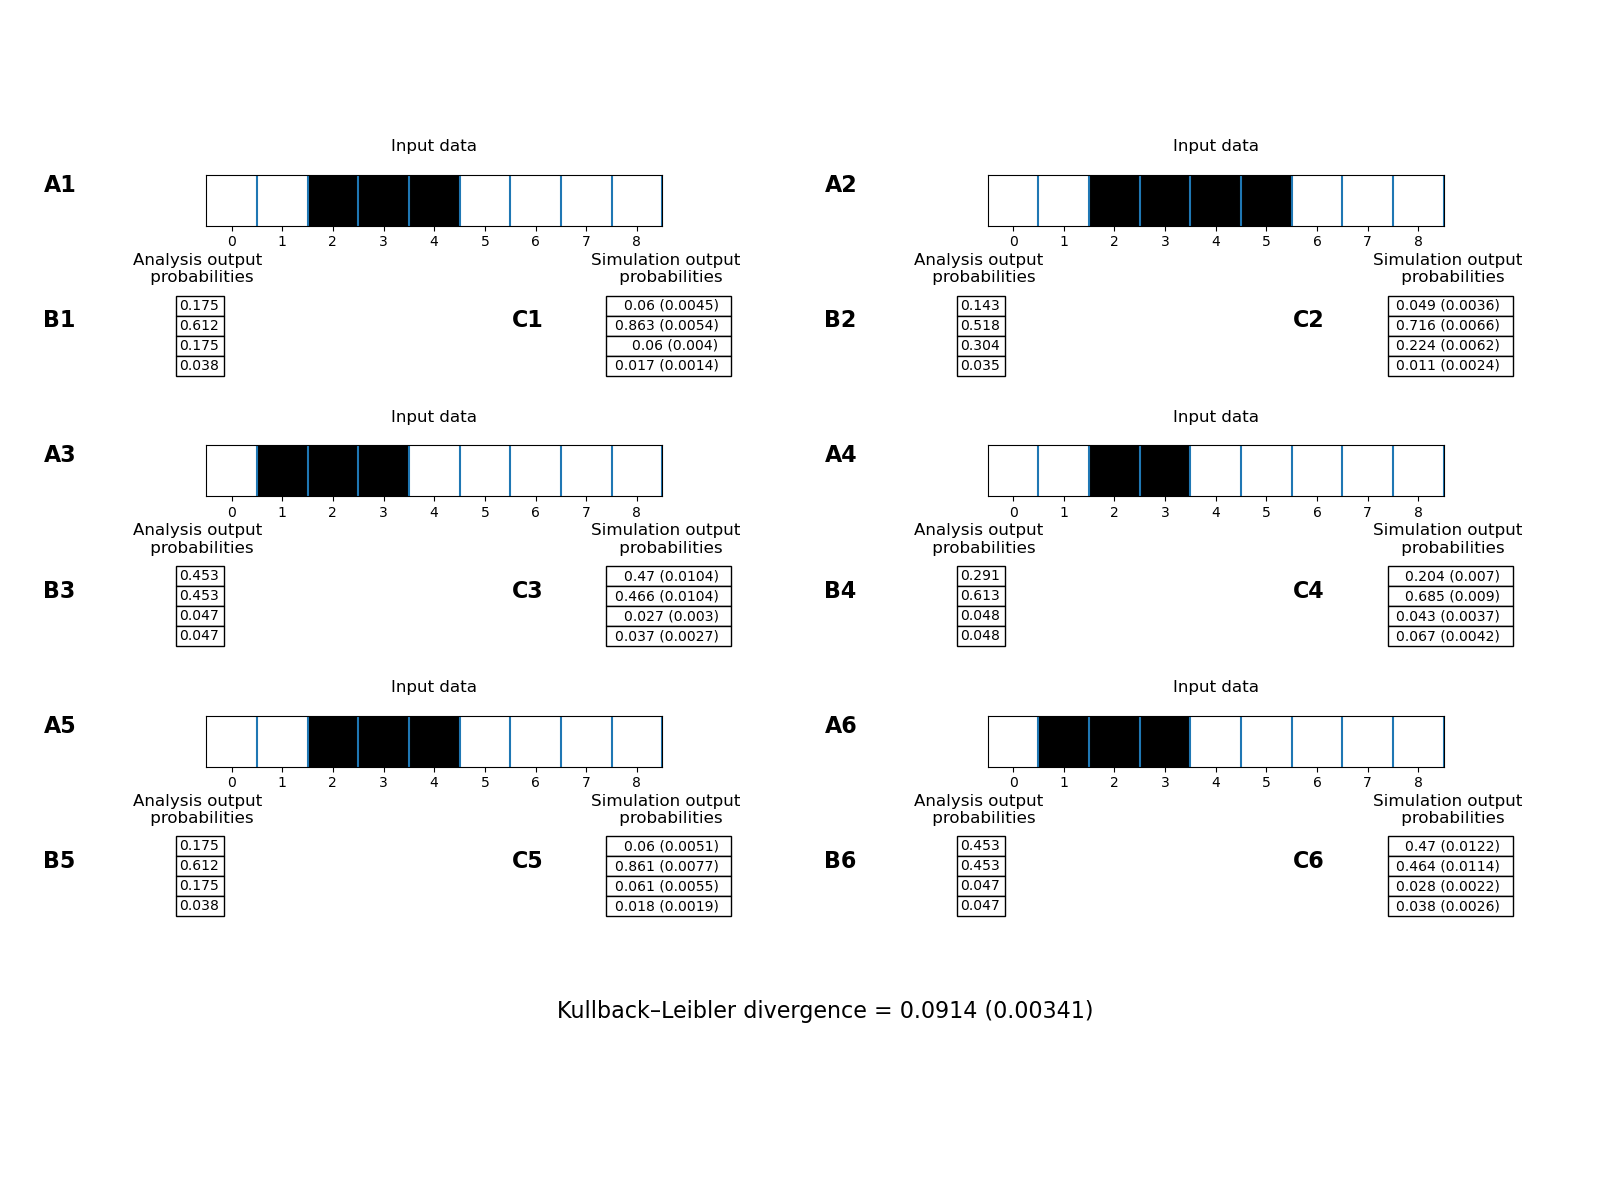
\includegraphics[width=\linewidth]{figures/1D/1D_70_0_15.png}
  \caption{\textbf{Analysis and simulation result. Parameters: }$f_{input} = 70 Hz, f_{prior} = 0 Hz, \tau_{decay} = 15 ms$ \textbf{A} Input images with 9 x 1 pixels. The red borders indicate the class of the prior. \textbf{B} Analytically calculated posterior probabilities. \textbf{C} Proportions of the spikes of the output neurons during the simulation and their standard deviations in brackets.}
  \label{fig:1D_70_0_15}
\end{figure}

\subparagraph{$\tau_{decay} = 0.004 seconds$, $f_{prior} = 0 Hz$}
For this parameter combination values between 50 and 150 Hz for $f_{input}$ in steps of 10 Hz were simulated. Analogously to the previous parameter set after finding the best input firing rate the search was performed in finer steps until the best value was determined as 88 Hz. The result of those parameters can be seen in Figure \ref{fig:1D_88_0_4}.

\begin{figure}
  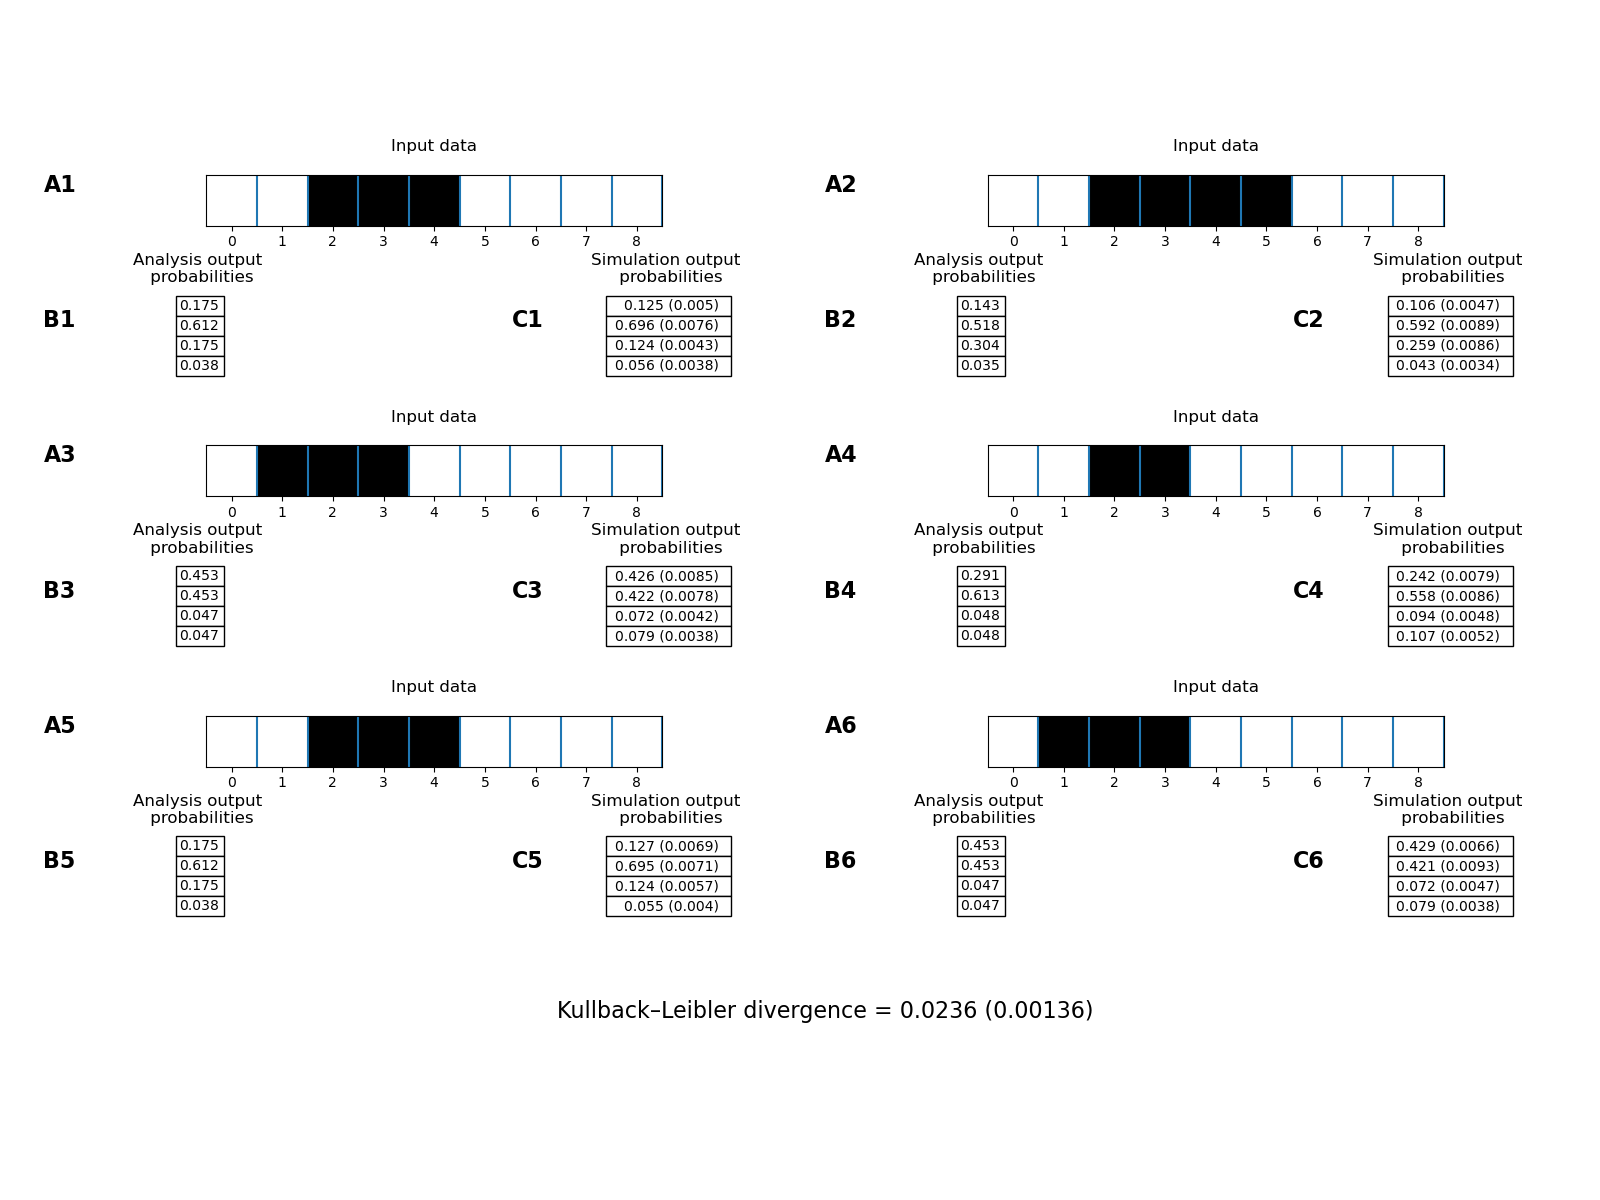
\includegraphics[width=\linewidth]{figures/1D/1D_88_0_4.png}
  \caption{\textbf{Analysis and simulation result. Parameters: } $f_{input} = 88 Hz, f_{prior} = 0 Hz, \tau_{decay} = 4 ms$ \textbf{A} Input images with 9 x 1 pixels. \textbf{B} Analytically calculated posterior probabilities. \textbf{C} Proportions of the spikes of the output neurons during the simulation and their standard deviations in brackets.}
  \label{fig:1D_88_0_4}
\end{figure}

\paragraph{Simulation results with prior}
After determining the best input firing rates for two different values of $\tau_{decay}$, the prior neurons were activated and the best prior firing rate $f_{prior}$ was fitted.
\subparagraph{$\tau_{decay} = 0.015 seconds$, $f_{input} = 42 Hz$}
The search for the best value of $f_{prior}$ was performed in the same manner as for $f_{input}$. Values between 140 and 240 Hz were simulated and a prior firing rate of 222 Hz performed the best. Its results can be seen in Figure \ref{fig:1D_42_222_15}. The value of the prior is indicated by the red border which is three pixels wide and centered at the center position of the corresponding output class.

\begin{figure}
  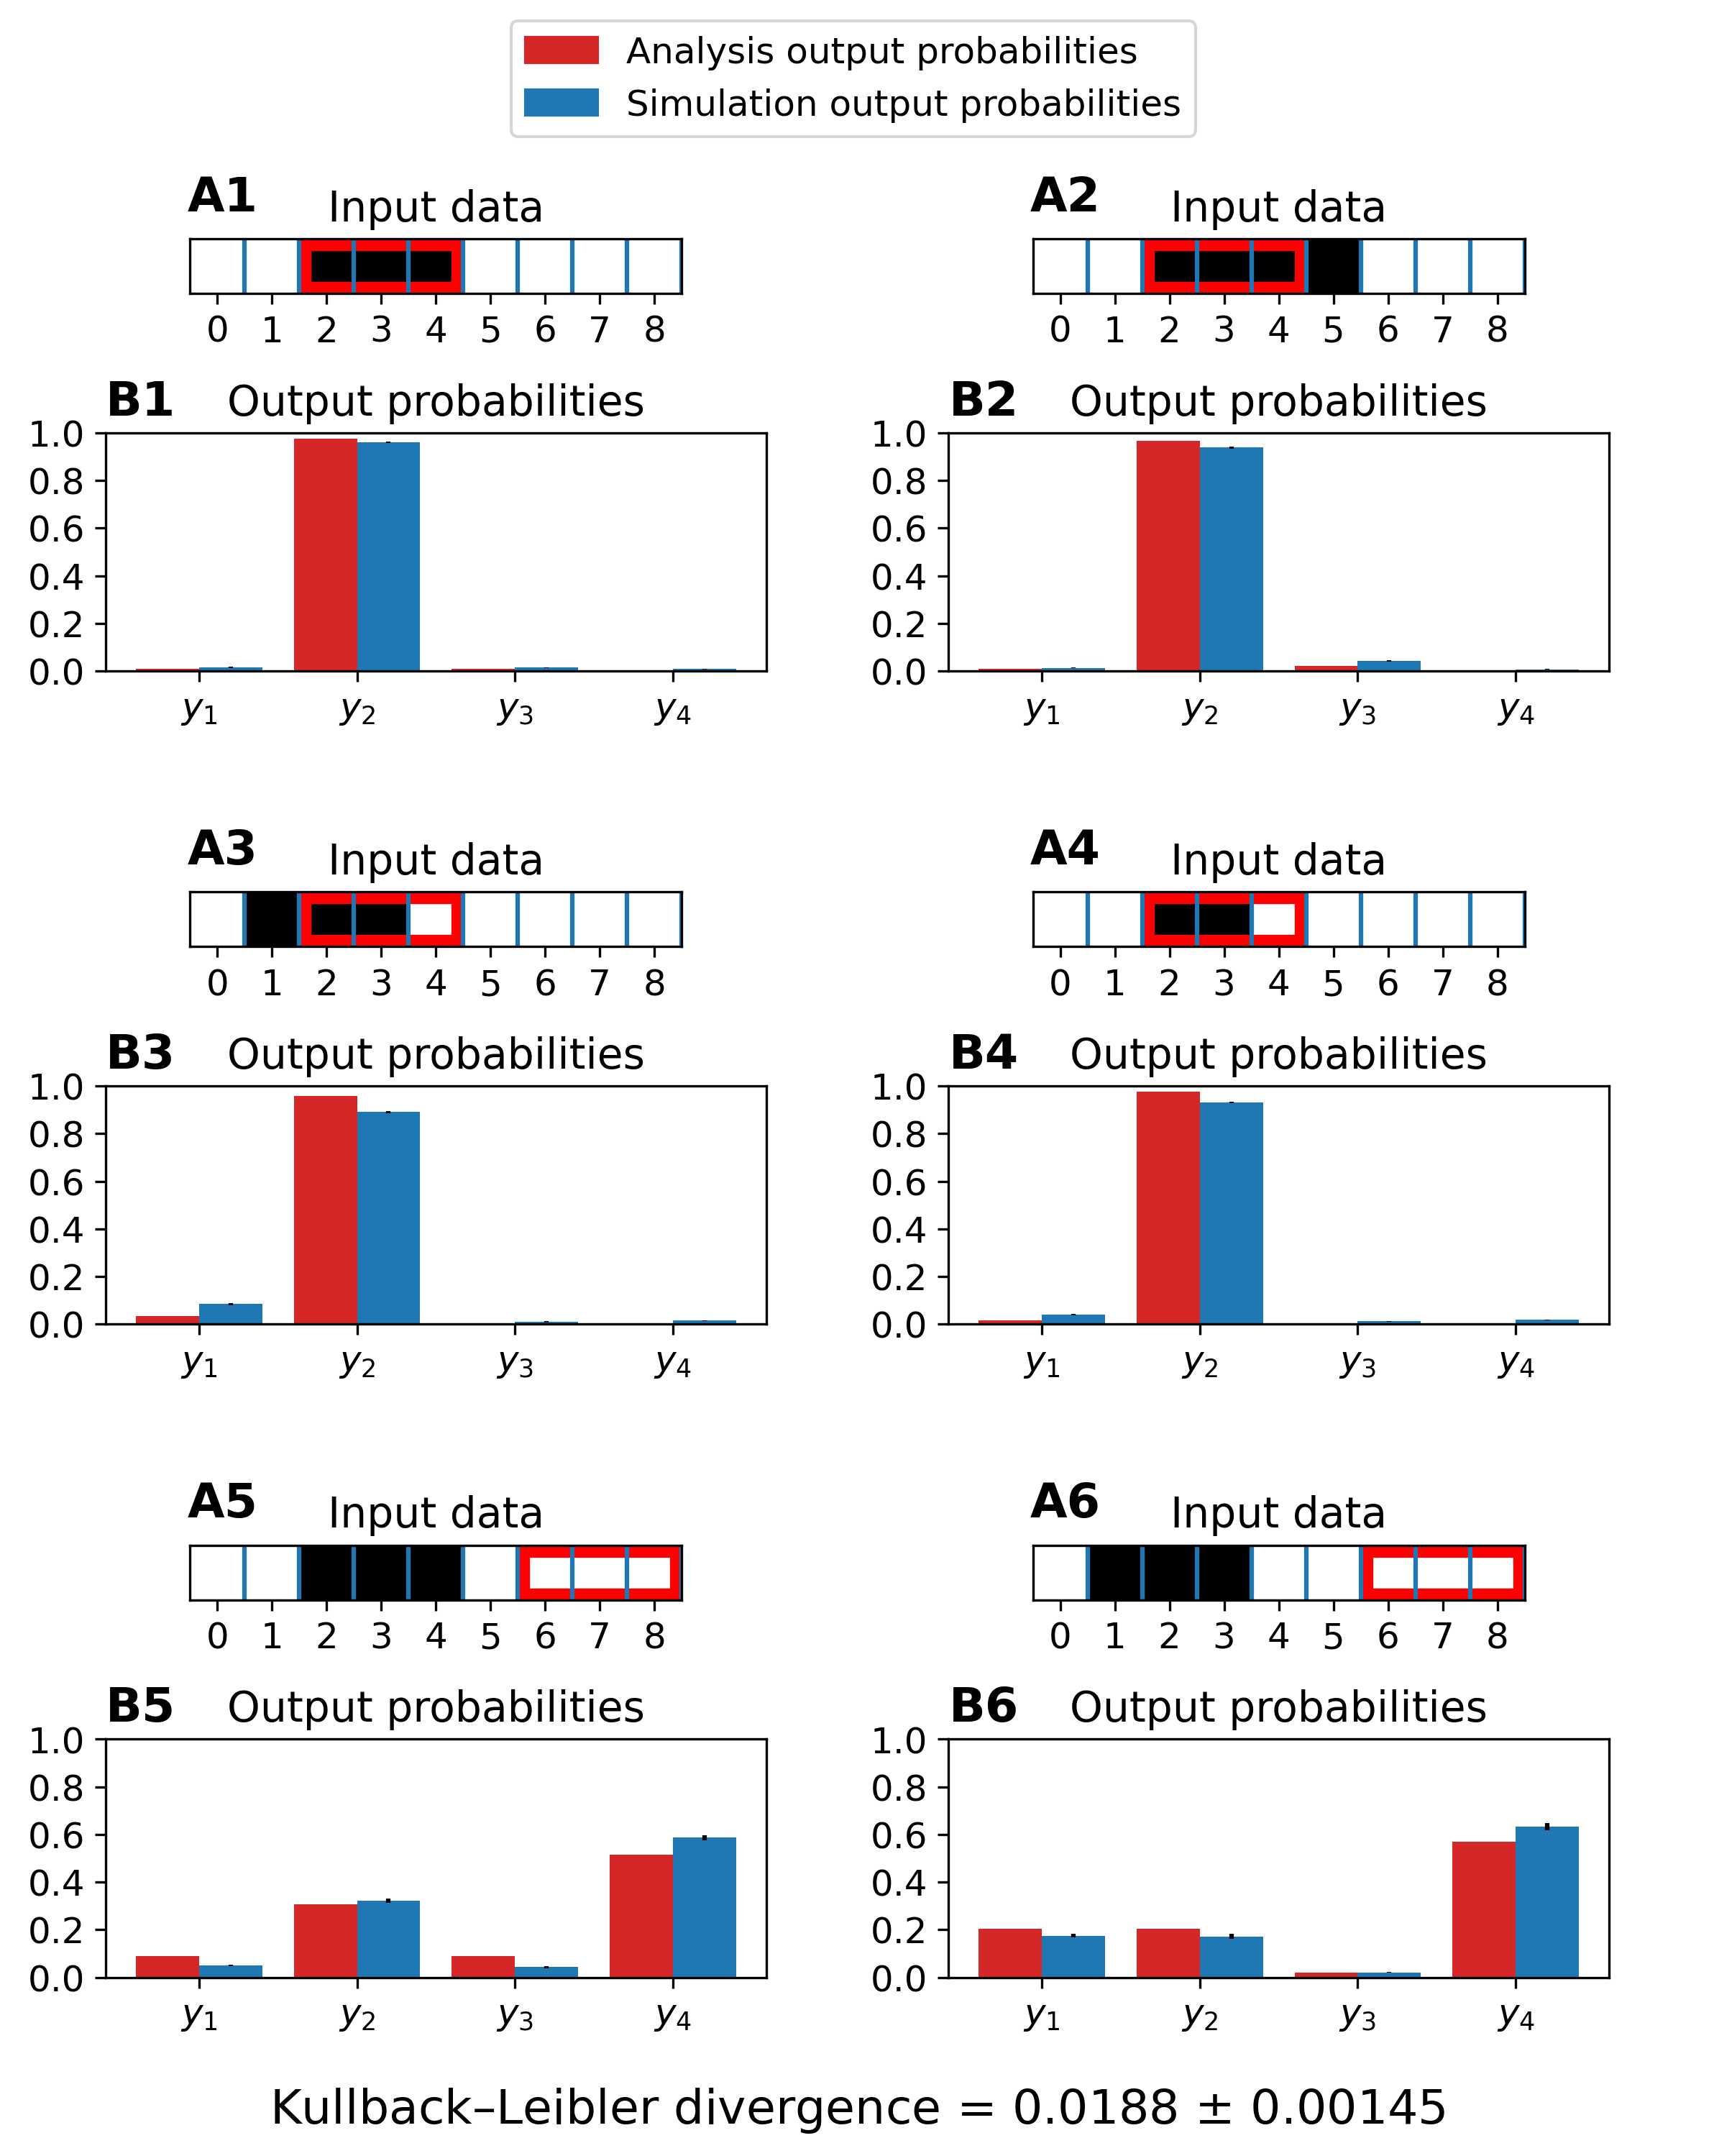
\includegraphics[width=\linewidth]{figures/1D/1D_42_222_15.png}
  \caption{\textbf{Analysis and simulation result. Parameters: } $f_{input} = 42 Hz, f_{prior} = 222 Hz, \tau_{decay} = 15 ms$ \textbf{A} Input images with 9 x 1 pixels. \textbf{B} Analytically calculated posterior probabilities. \textbf{C} Proportions of the spikes of the output neurons during the simulation and their standard deviations in brackets.}
  \label{fig:1D_42_222_15}
\end{figure}

\subparagraph{$\tau_{decay} = 0.004 seconds$, $f_{input} = 88 Hz$}
The search for the best value of $f_{prior}$ was performed in the same manner as for $f_{input}$. Values between 360 and 460 Hz were simulated and a prior firing rate of 440 Hz performed the best. The results of this parameter combination are given in Figure \ref{fig:1D_88_440_4}.

\begin{figure}
  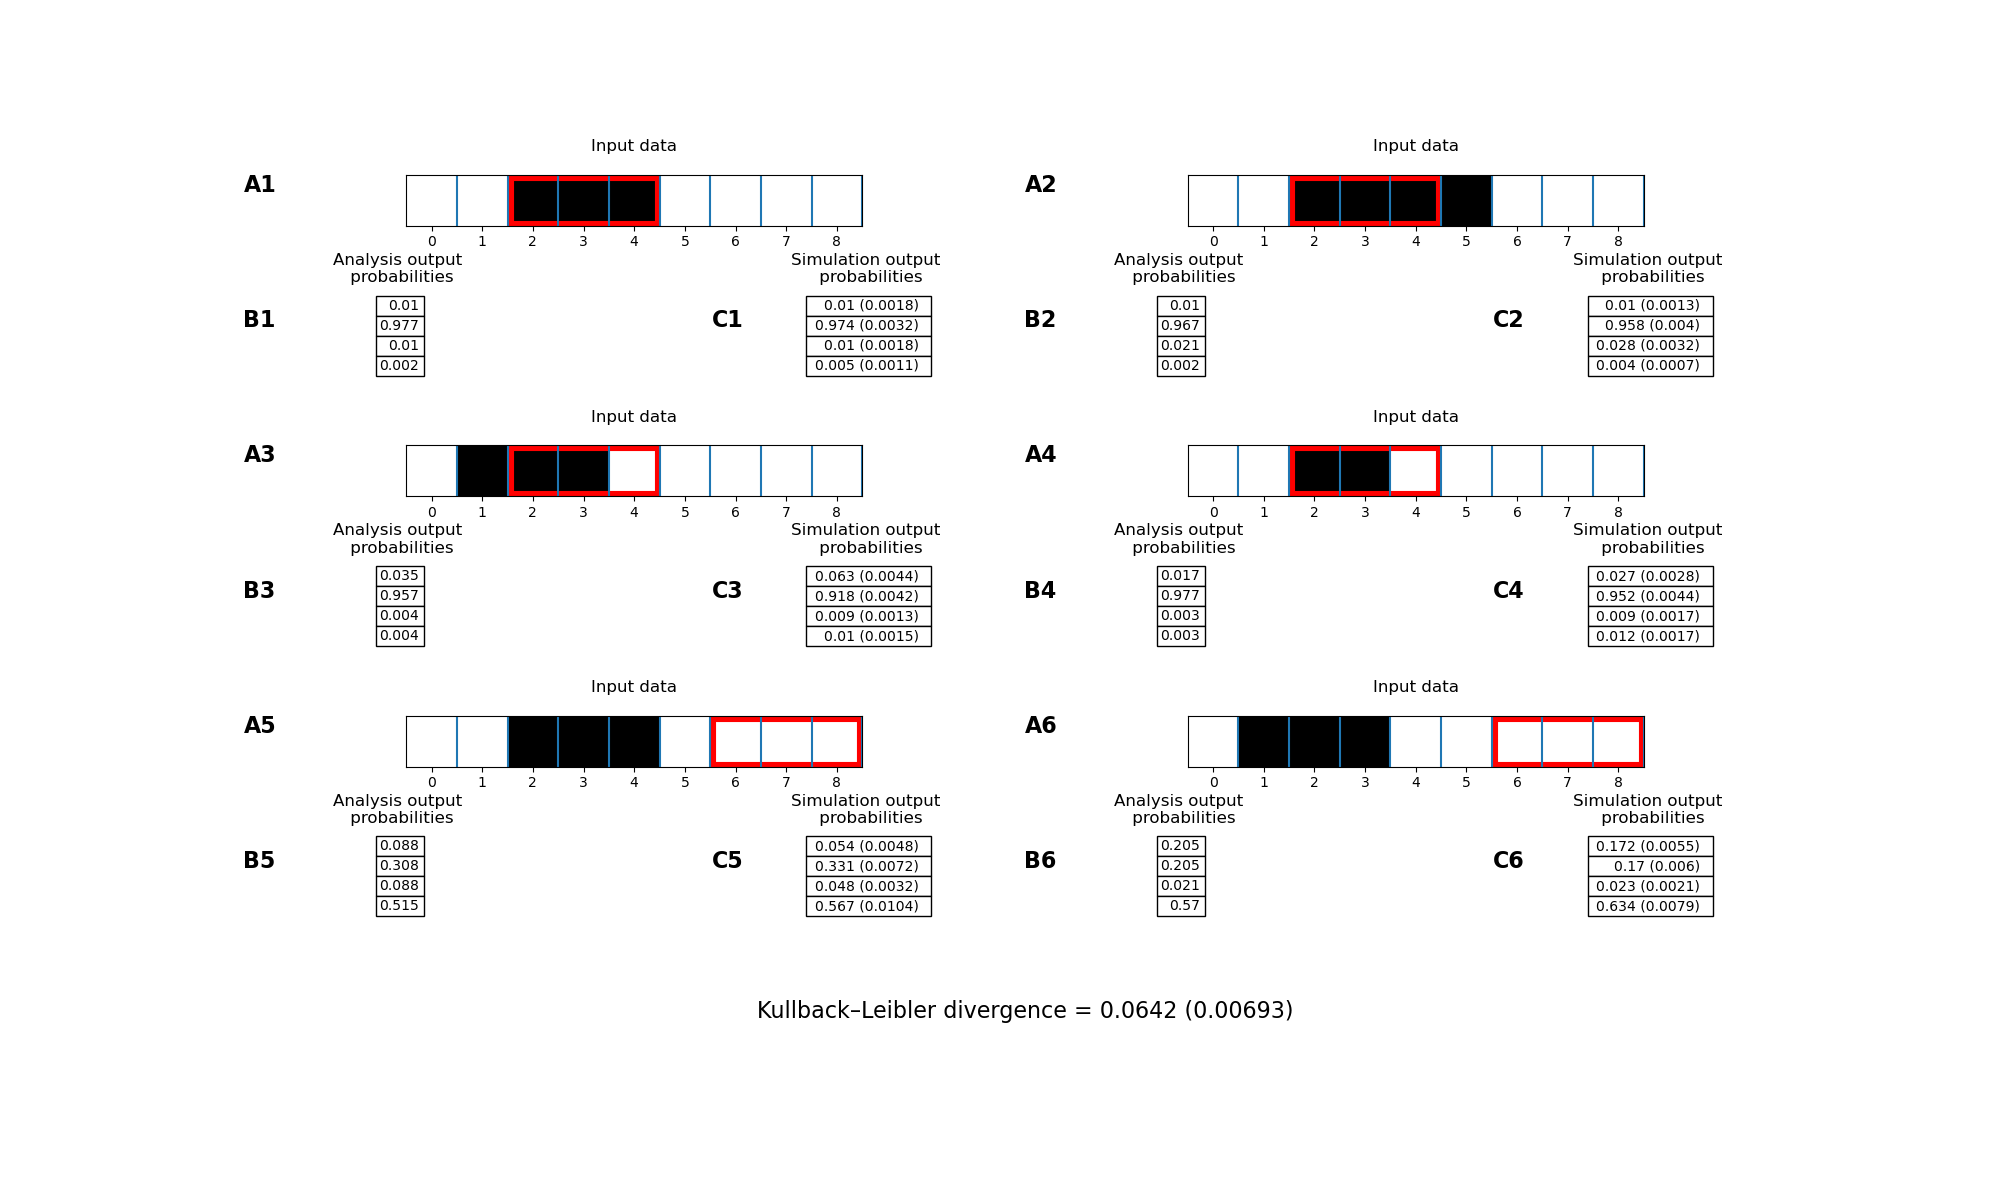
\includegraphics[width=\linewidth]{figures/1D/1D_88_440_4.png}
  \caption{\textbf{Analysis and simulation result. Parameters: } $f_{input} = 88 Hz, f_{prior} = 440 Hz, \tau_{decay} = 4 ms$ \textbf{A} Input images with 9 x 1 pixels. \textbf{B} Analytically calculated posterior probabilities. \textbf{C} Proportions of the spikes of the output neurons during the simulation and their standard deviations in brackets.}
  \label{fig:1D_88_440_4}
\end{figure}

To demonstrate the impact of rising $f_{prior}$ it was set to 600 Hz and the results can be seen in Figure \ref{fig:1D_88_600_4}.

\begin{figure}
  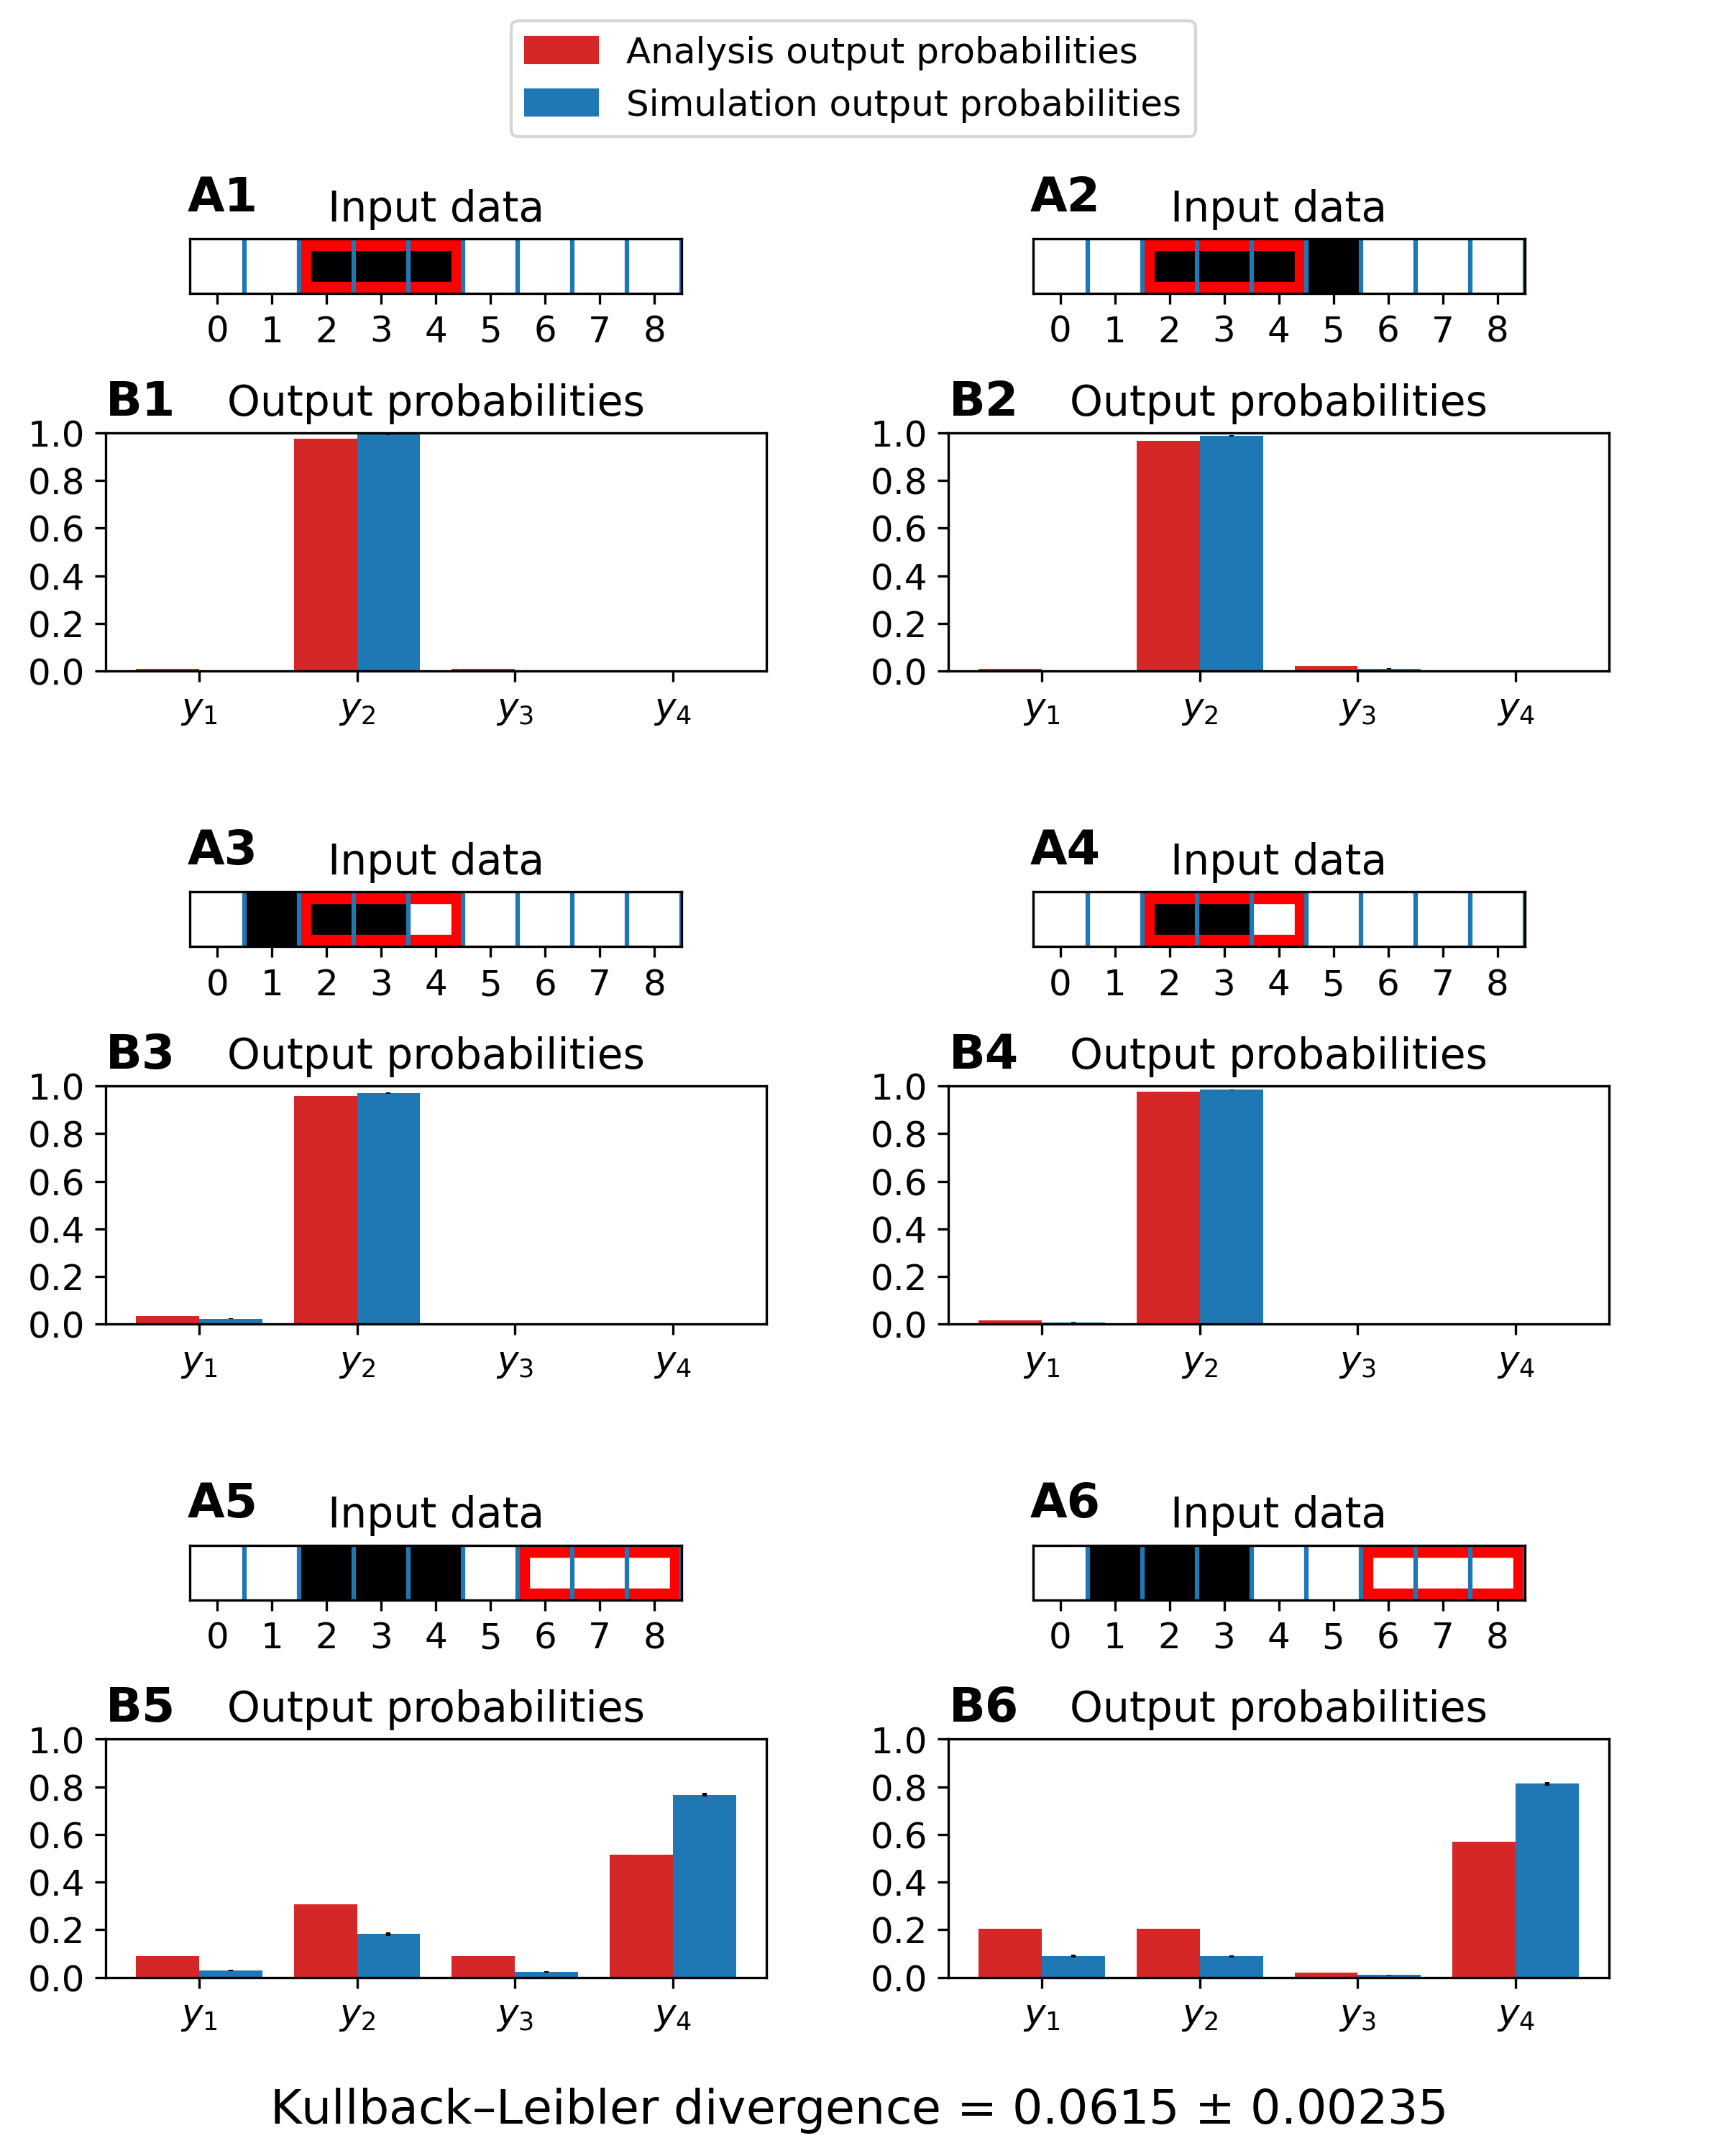
\includegraphics[width=\linewidth]{figures/1D/1D_88_600_4.png}
  \caption{\textbf{Analysis and simulation result. The Kullback-Leibler divergence could not be calculated for this case, as it is not defined for probabilities of 0. Parameters: } $f_{input} = 88 Hz, f_{prior} = 600 Hz, \tau_{decay} = 4 ms$ \textbf{A} Input images with 9 x 1 pixels. \textbf{B} Analytically calculated posterior probabilities. \textbf{C} Proportions of the spikes of the output neurons during the simulation and their standard deviations in brackets.}
  \label{fig:1D_88_600_4}
\end{figure}

\subparagraph{$\tau_{decay} = 0.004 seconds$, $f_{input} = 98$, $f_{prior} = 440 Hz$}
Finally to it was tested if a increase of $f_{input}$ might decrease the Kullback-Leibler divergence even further. The network was simulated with increasing values of $f_{input}$ in steps of 2 Hz, beginning from 90 Hz. The best result was obtained with an input firing rate of 98 Hz. The results of that simulation can be seen in Figure \ref{fig:1D_98_440_4}.

\begin{figure}
  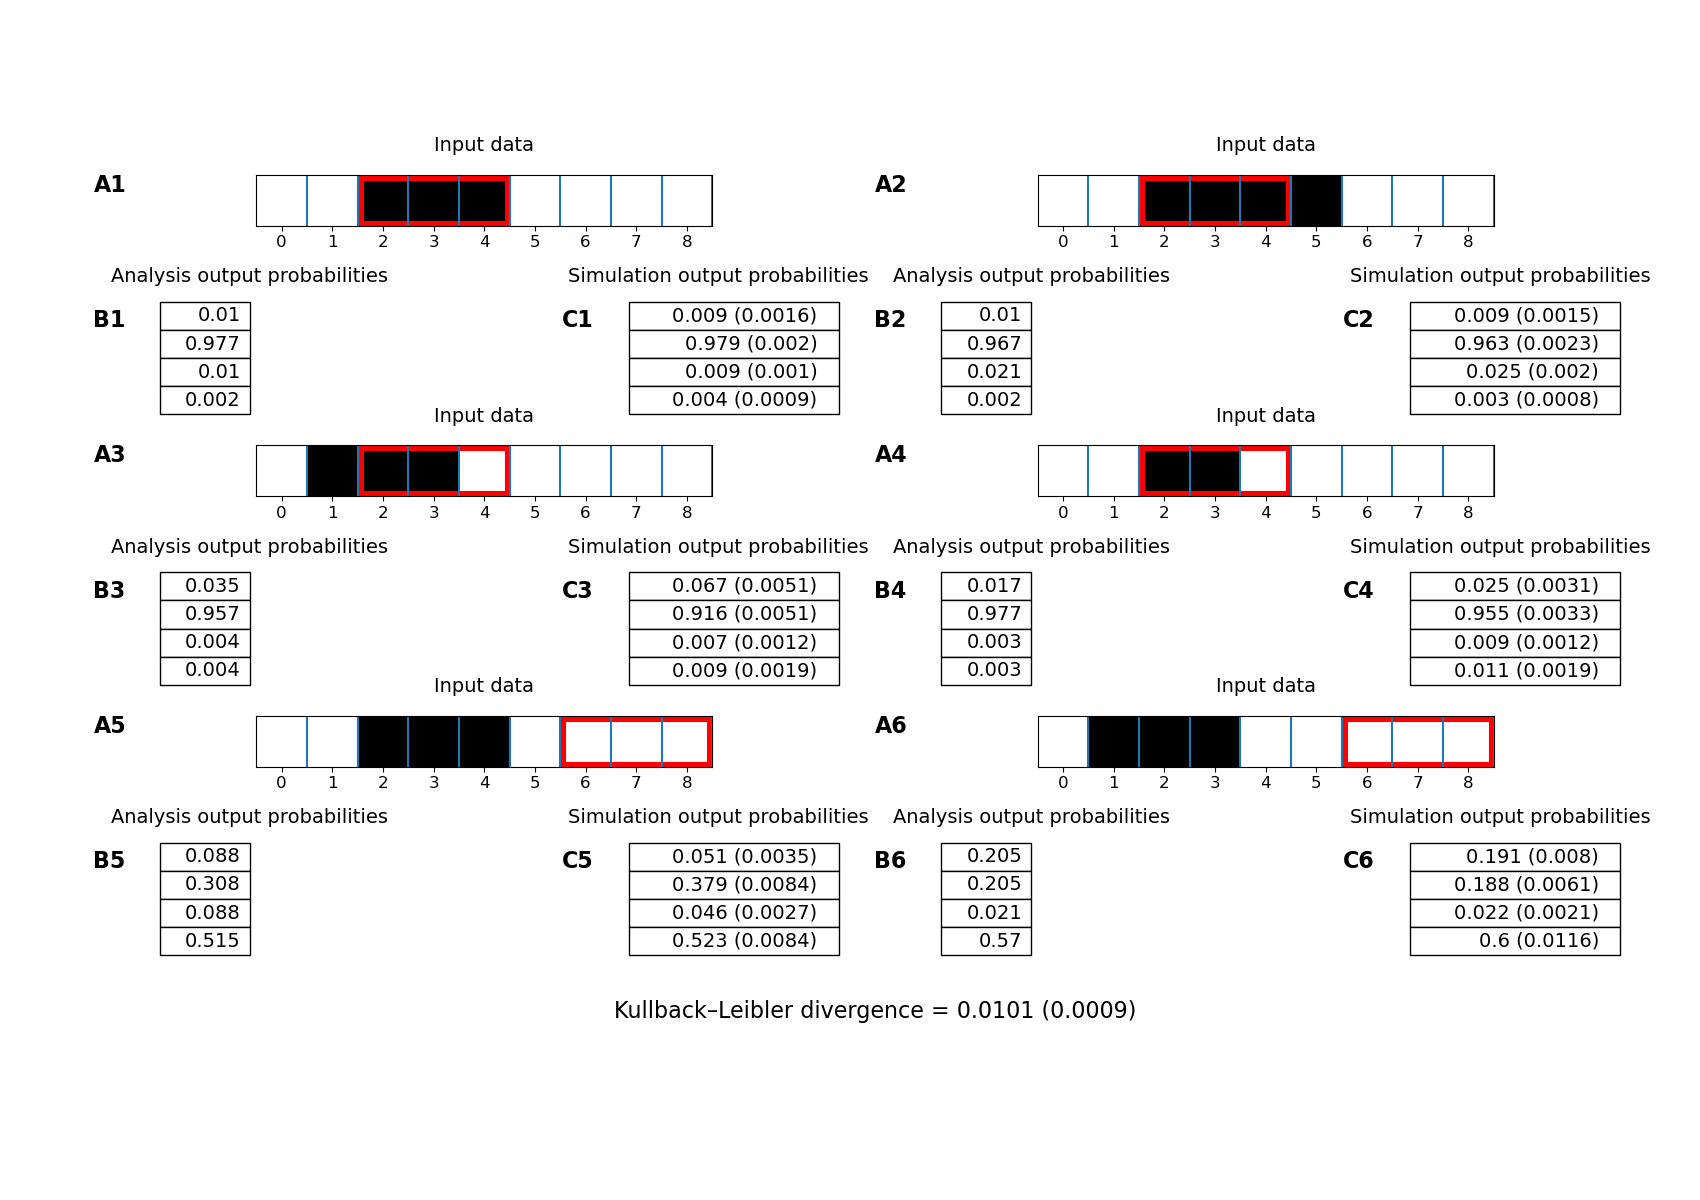
\includegraphics[width=\linewidth]{figures/1D/1D_98_440_4.png}
  \caption{\textbf{Analysis and simulation result. Parameters: } $f_{input} = 98 Hz, f_{prior} = 440 Hz, \tau_{decay} = 4 ms$ \textbf{A} Input images with 9 x 1 pixels. \textbf{B} Analytically calculated posterior probabilities. \textbf{C} Proportions of the spikes of the output neurons during the simulation and their standard deviations in brackets.}
  \label{fig:1D_98_440_4}
\end{figure}

\subsection{Discussion}

In this experiment the impact of the three network parameters $f_{input}$, $f_{prior}$ and $\tau_{decay}$ was analysed.

\paragraph{$f_{input}$} controls how strongly the information of the pixels of the input image is weighed. This means that by raising $f_{input}$ the impact of the active pixels increases, while the impact of the prior neuron decreases comparatively. This effect will be shown in the discussion about $f_{prior}$. However this is not the only impact this parameter has. When raising $f_{input}$ it was also observed that the probabilities for output classes adjacent to the active pixels decreased. This can be observed when comparing Figures \ref{fig:1D_42_0_15} and \ref{fig:1D_70_0_15} where $f_{input}$ was raised from 42 Hz to 70 Hz. For example when looking at "C4" in the mentioned figures, it can be seen that for $f_{input} = 42 Hz$ the simulation output probability for class 1 is 0.245. This high probability is mostly due to the active pixel number 2, which belongs to class 1 and 2 at the same time. When now increasing $f_{input}$ to 70 Hz one might expect the probabilities for class 1 and 2 to rise. This however does not happen, instead the simulation output probability for class 1 fell to 0.207, while for class 2 it rose.
It is assumed that this happens because the membrane potentials of the output neurons are never normalized. As the input neurons spike more quickly the membrane potential of output neuron 1 rises slower than the membrane potential of output neuron 2. This leads to shifted firing rates in favour of output neuron 2. However this behaviour might be expected, as faster spiking input neurons correspond statistically to taking more samples of a probability distribution. This means that the more samples the network takes, the more certain it becomes of the more likely option, which is output class 2.

\paragraph{$f_{prior}$} When increasing the prior firing rate the impact on the result of the prior neurons increases, while the impact of the input neurons decreases comparatively. When comparing the Figures \ref{fig:1D_88_440_4} and \ref{fig:1D_88_600_4} which show the results for $f_{input} = 88 Hz$, $\tau_{decay} = 4 ms$ and $f_{prior} = 440$ and $600 Hz$ respectively it can be seen under "C6" how the probability for output class 4 rose, while all other probabilities fell. The opposite behaviour can be observed when raising $f_{input}$ instead, but no separate figure will be provided for this case.

\paragraph{$\tau_{decay}$} determines for how long and how strongly an input or prior spike contributes to the membrane potentials of the output neurons. The bigger $\tau_{decay}$ is, the smaller $f_{input}$ and $f_{prior}$ need to be, to minimize the Kullback-Leibler divergence. This is represented by the final parameters for $\tau_{decay}$ of 4 and 15 ms. While for $\tau_{decay} = 15 ms$ the best input firing rate was 42 Hz and the prior firing rate was 222 Hz, for $\tau_{decay} = 4 ms$ they had to be raised to 98 and 440 Hz to minimize the Kullback-Leibler divergence.

\paragraph{Approximating the analytic solution}
After first finding the optimal $f_{input}$ for disabled prior activity and then finding the optimal $f_{prior}$ with enabled prior activity for $\tau_{decay}$ the simulation was not yet approximating the analytical solution perfectly. Because of that it was tried to raise $f_{input}$ to further decrease the Kullback-Leibler divergence. The further search for a better $f_{input}$ was performed for $\tau_{decay} = 0.004 ms$ and $f_{prior} = 440 Hz$, as this set of parameters performed the best overall.
When comparing the former optimal result in Figure \ref{fig:1D_88_440_4} with $f_{input} = 88 Hz$, to the result with $f_{input} = 98 Hz$ in Figure \ref{fig:1D_98_440_4}, it can be seen that the Kullback-Leibler divergence decreased from 0.0112 to 0.0101. The simulation output probabilities with the higher $f_{input}$ approximated the analysis output probabilities for example for "B3" and "C3" in the mentioned figures on one hand better, while on the other hand for "B5" and "C5" the output probabilities of the analysis and the simulation of class 2 diverged more. A further increase of $f_{input}$ started to increase the Kullback-Leibler divergence again, thus the final optimum of the parameter set was reached. It is assumed that increasing $f_{input}$ after $f_{prior}$ was fitted was necessary because the proportion of the impact of $f_{input}$ on the simulation decreased due to the introduction of the prior activity.

\section{Experiment 5: Simulation of the 1D network with double size}
\label{section:1DDoubleSize}

\subsection{Introduction}

\subsection{Methods}

\subsection{Results}

\subsection{Discussion}

\section{Experiment 6: Training of the 1D network with predetermined parameters}
\label{section:1DDoubleSize}

\subsection{Introduction}

\subsection{Methods}

\subsection{Results}

\subsection{Discussion}